% Options for packages loaded elsewhere
\PassOptionsToPackage{unicode}{hyperref}
\PassOptionsToPackage{hyphens}{url}
\PassOptionsToPackage{dvipsnames,svgnames,x11names}{xcolor}
%
\documentclass[
  number]{elsarticle}

\usepackage{amsmath,amssymb}
\usepackage{iftex}
\ifPDFTeX
  \usepackage[T1]{fontenc}
  \usepackage[utf8]{inputenc}
  \usepackage{textcomp} % provide euro and other symbols
\else % if luatex or xetex
  \usepackage{unicode-math}
  \defaultfontfeatures{Scale=MatchLowercase}
  \defaultfontfeatures[\rmfamily]{Ligatures=TeX,Scale=1}
\fi
\usepackage{lmodern}
\ifPDFTeX\else  
    % xetex/luatex font selection
\fi
% Use upquote if available, for straight quotes in verbatim environments
\IfFileExists{upquote.sty}{\usepackage{upquote}}{}
\IfFileExists{microtype.sty}{% use microtype if available
  \usepackage[]{microtype}
  \UseMicrotypeSet[protrusion]{basicmath} % disable protrusion for tt fonts
}{}
\makeatletter
\@ifundefined{KOMAClassName}{% if non-KOMA class
  \IfFileExists{parskip.sty}{%
    \usepackage{parskip}
  }{% else
    \setlength{\parindent}{0pt}
    \setlength{\parskip}{6pt plus 2pt minus 1pt}}
}{% if KOMA class
  \KOMAoptions{parskip=half}}
\makeatother
\usepackage{xcolor}
\setlength{\emergencystretch}{3em} % prevent overfull lines
\setcounter{secnumdepth}{-\maxdimen} % remove section numbering
% Make \paragraph and \subparagraph free-standing
\makeatletter
\ifx\paragraph\undefined\else
  \let\oldparagraph\paragraph
  \renewcommand{\paragraph}{
    \@ifstar
      \xxxParagraphStar
      \xxxParagraphNoStar
  }
  \newcommand{\xxxParagraphStar}[1]{\oldparagraph*{#1}\mbox{}}
  \newcommand{\xxxParagraphNoStar}[1]{\oldparagraph{#1}\mbox{}}
\fi
\ifx\subparagraph\undefined\else
  \let\oldsubparagraph\subparagraph
  \renewcommand{\subparagraph}{
    \@ifstar
      \xxxSubParagraphStar
      \xxxSubParagraphNoStar
  }
  \newcommand{\xxxSubParagraphStar}[1]{\oldsubparagraph*{#1}\mbox{}}
  \newcommand{\xxxSubParagraphNoStar}[1]{\oldsubparagraph{#1}\mbox{}}
\fi
\makeatother

\usepackage{color}
\usepackage{fancyvrb}
\newcommand{\VerbBar}{|}
\newcommand{\VERB}{\Verb[commandchars=\\\{\}]}
\DefineVerbatimEnvironment{Highlighting}{Verbatim}{commandchars=\\\{\}}
% Add ',fontsize=\small' for more characters per line
\usepackage{framed}
\definecolor{shadecolor}{RGB}{241,243,245}
\newenvironment{Shaded}{\begin{snugshade}}{\end{snugshade}}
\newcommand{\AlertTok}[1]{\textcolor[rgb]{0.68,0.00,0.00}{#1}}
\newcommand{\AnnotationTok}[1]{\textcolor[rgb]{0.37,0.37,0.37}{#1}}
\newcommand{\AttributeTok}[1]{\textcolor[rgb]{0.40,0.45,0.13}{#1}}
\newcommand{\BaseNTok}[1]{\textcolor[rgb]{0.68,0.00,0.00}{#1}}
\newcommand{\BuiltInTok}[1]{\textcolor[rgb]{0.00,0.23,0.31}{#1}}
\newcommand{\CharTok}[1]{\textcolor[rgb]{0.13,0.47,0.30}{#1}}
\newcommand{\CommentTok}[1]{\textcolor[rgb]{0.37,0.37,0.37}{#1}}
\newcommand{\CommentVarTok}[1]{\textcolor[rgb]{0.37,0.37,0.37}{\textit{#1}}}
\newcommand{\ConstantTok}[1]{\textcolor[rgb]{0.56,0.35,0.01}{#1}}
\newcommand{\ControlFlowTok}[1]{\textcolor[rgb]{0.00,0.23,0.31}{\textbf{#1}}}
\newcommand{\DataTypeTok}[1]{\textcolor[rgb]{0.68,0.00,0.00}{#1}}
\newcommand{\DecValTok}[1]{\textcolor[rgb]{0.68,0.00,0.00}{#1}}
\newcommand{\DocumentationTok}[1]{\textcolor[rgb]{0.37,0.37,0.37}{\textit{#1}}}
\newcommand{\ErrorTok}[1]{\textcolor[rgb]{0.68,0.00,0.00}{#1}}
\newcommand{\ExtensionTok}[1]{\textcolor[rgb]{0.00,0.23,0.31}{#1}}
\newcommand{\FloatTok}[1]{\textcolor[rgb]{0.68,0.00,0.00}{#1}}
\newcommand{\FunctionTok}[1]{\textcolor[rgb]{0.28,0.35,0.67}{#1}}
\newcommand{\ImportTok}[1]{\textcolor[rgb]{0.00,0.46,0.62}{#1}}
\newcommand{\InformationTok}[1]{\textcolor[rgb]{0.37,0.37,0.37}{#1}}
\newcommand{\KeywordTok}[1]{\textcolor[rgb]{0.00,0.23,0.31}{\textbf{#1}}}
\newcommand{\NormalTok}[1]{\textcolor[rgb]{0.00,0.23,0.31}{#1}}
\newcommand{\OperatorTok}[1]{\textcolor[rgb]{0.37,0.37,0.37}{#1}}
\newcommand{\OtherTok}[1]{\textcolor[rgb]{0.00,0.23,0.31}{#1}}
\newcommand{\PreprocessorTok}[1]{\textcolor[rgb]{0.68,0.00,0.00}{#1}}
\newcommand{\RegionMarkerTok}[1]{\textcolor[rgb]{0.00,0.23,0.31}{#1}}
\newcommand{\SpecialCharTok}[1]{\textcolor[rgb]{0.37,0.37,0.37}{#1}}
\newcommand{\SpecialStringTok}[1]{\textcolor[rgb]{0.13,0.47,0.30}{#1}}
\newcommand{\StringTok}[1]{\textcolor[rgb]{0.13,0.47,0.30}{#1}}
\newcommand{\VariableTok}[1]{\textcolor[rgb]{0.07,0.07,0.07}{#1}}
\newcommand{\VerbatimStringTok}[1]{\textcolor[rgb]{0.13,0.47,0.30}{#1}}
\newcommand{\WarningTok}[1]{\textcolor[rgb]{0.37,0.37,0.37}{\textit{#1}}}

\providecommand{\tightlist}{%
  \setlength{\itemsep}{0pt}\setlength{\parskip}{0pt}}\usepackage{longtable,booktabs,array}
\usepackage{calc} % for calculating minipage widths
% Correct order of tables after \paragraph or \subparagraph
\usepackage{etoolbox}
\makeatletter
\patchcmd\longtable{\par}{\if@noskipsec\mbox{}\fi\par}{}{}
\makeatother
% Allow footnotes in longtable head/foot
\IfFileExists{footnotehyper.sty}{\usepackage{footnotehyper}}{\usepackage{footnote}}
\makesavenoteenv{longtable}
\usepackage{graphicx}
\makeatletter
\newsavebox\pandoc@box
\newcommand*\pandocbounded[1]{% scales image to fit in text height/width
  \sbox\pandoc@box{#1}%
  \Gscale@div\@tempa{\textheight}{\dimexpr\ht\pandoc@box+\dp\pandoc@box\relax}%
  \Gscale@div\@tempb{\linewidth}{\wd\pandoc@box}%
  \ifdim\@tempb\p@<\@tempa\p@\let\@tempa\@tempb\fi% select the smaller of both
  \ifdim\@tempa\p@<\p@\scalebox{\@tempa}{\usebox\pandoc@box}%
  \else\usebox{\pandoc@box}%
  \fi%
}
% Set default figure placement to htbp
\def\fps@figure{htbp}
\makeatother

\usepackage{booktabs}
\usepackage{caption}
\usepackage{longtable}
\usepackage{colortbl}
\usepackage{array}
\usepackage{anyfontsize}
\usepackage{multirow}
\usepackage[a4paper, margin=1in]{geometry}
\makeatletter
\@ifpackageloaded{caption}{}{\usepackage{caption}}
\AtBeginDocument{%
\ifdefined\contentsname
  \renewcommand*\contentsname{Table of contents}
\else
  \newcommand\contentsname{Table of contents}
\fi
\ifdefined\listfigurename
  \renewcommand*\listfigurename{List of Figures}
\else
  \newcommand\listfigurename{List of Figures}
\fi
\ifdefined\listtablename
  \renewcommand*\listtablename{List of Tables}
\else
  \newcommand\listtablename{List of Tables}
\fi
\ifdefined\figurename
  \renewcommand*\figurename{Figure}
\else
  \newcommand\figurename{Figure}
\fi
\ifdefined\tablename
  \renewcommand*\tablename{Table}
\else
  \newcommand\tablename{Table}
\fi
}
\@ifpackageloaded{float}{}{\usepackage{float}}
\floatstyle{ruled}
\@ifundefined{c@chapter}{\newfloat{codelisting}{h}{lop}}{\newfloat{codelisting}{h}{lop}[chapter]}
\floatname{codelisting}{Listing}
\newcommand*\listoflistings{\listof{codelisting}{List of Listings}}
\makeatother
\makeatletter
\usepackage{pdflscape}
\makeatother
\makeatletter
\makeatother
\makeatletter
\@ifpackageloaded{caption}{}{\usepackage{caption}}
\@ifpackageloaded{subcaption}{}{\usepackage{subcaption}}
\makeatother
\journal{Data in Brief}

\usepackage[]{natbib}
\bibliographystyle{elsarticle-num}
\usepackage{bookmark}

\IfFileExists{xurl.sty}{\usepackage{xurl}}{} % add URL line breaks if available
\urlstyle{same} % disable monospaced font for URLs
\hypersetup{
  pdftitle={From Archives to AI: Residential Property Data Across Three Decades in Brunei Darussalam},
  pdfkeywords={Housing Market, Brunei, Property Listings, Spatial
Data, Web Scraping, Large Language Models},
  colorlinks=true,
  linkcolor={blue},
  filecolor={Maroon},
  citecolor={Blue},
  urlcolor={Blue},
  pdfcreator={LaTeX via pandoc}}


\setlength{\parindent}{6pt}
\begin{document}

\begin{frontmatter}
\title{From Archives to AI: Residential Property Data Across Three
Decades in Brunei Darussalam}
\author[1]{Haziq Jamil%
\corref{cor1}%
}
 \ead{haziq.jamil@ubd.edu.bn} 
\author[1]{Amira Barizah Noorosmawie%
%
}

\author[1]{Hafeezul Waezz Rabu%
%
}

\author[2]{Lutfi Abdul Razak%
%
}
 \ead{lutfi.razak@ubd.edu.bn} 

\affiliation[1]{organization={Universiti Brunei Darussalam, Mathematical
Sciences, Faculty of Science},addressline={Universiti Brunei Darussalam,
Jalan Tungku Link},city={Bandar Seri
Begawan},country={Brunei},countrysep={,},postcode={BE
1410},postcodesep={}}
\affiliation[2]{organization={UBD School of Business and
Economics},addressline={Universiti Brunei Darussalam, Jalan Tungku
Link},city={Bandar Seri
Begawan},country={Brunei},countrysep={,},postcode={BE
1410},postcodesep={}}

\cortext[cor1]{Corresponding author}




        
% Add manuscript URL
\makeatletter
\def\@elsuads{\url{https://bruneiverse.github.io/house-data}}
\makeatother

\begin{abstract}
This article introduces the first publicly available data set for
analysing the Brunei housing market, covering more than 30,000 property
listings from 1993 to early 2025. The data set, curated from property
advertisements in newspapers and online platforms, includes key
attributes such as price, location, property type, and physical
characteristics, enriched with area-level spatial information.
Comprehensive and historical, it complements the Brunei Darussalam
Central Bank's Residential Property Price Index (RPPI), addressing the
limitations of restricted access to raw RPPI data and its relatively
short timeline since its inception in 2015. Data collection involved
manual transcription from archival sources and automated web scraping
using programmatic techniques, supported by innovative processing with
Large Language Models (LLMs) to codify unstructured text. The data set
enables spatial and temporal analysis, with potential applications in
economics, urban planning, and real estate research. Although listing
prices are only a proxy for market values and may deviate from actual
sale prices due to negotiation dynamics and other factors, this data set
still provides a valuable resource for quantitative analyses of housing
market trends and for informing policy decisions.
\end{abstract}





\begin{keyword}
    Housing Market \sep Brunei \sep Property Listings \sep Spatial
Data \sep Web Scraping \sep 
    Large Language Models
\end{keyword}
\end{frontmatter}
    

\section{Citation}\label{citation}

For attribution, please cite this work as:

\begin{quote}
H. Jamil, A.B. Noorosmawie, H.W. Rabu, L. Abdul Razak, From Archives to
AI: Residential Property Data Across Three Decades in Brunei Darussalam,
Data in Brief (2025). \url{https://doi.org/10.1016/j.dib.2025.111505}.
\end{quote}

\section{Value of the Data}\label{value-of-the-data}

\begin{itemize}
\item
  \textbf{A first-of-its-kind data set for Brunei}. This data set is the
  first publicly available compilation of Brunei's residential property
  data, covering 31,116 listings from 1993 to early 2025. Previous
  studies on Brunei's housing have either relied on recent or
  non-spatial data \citep{ng2022characterising, jamil2025leveraging}, or
  have primarily employed qualitative methods due to the absence of
  structured data \citep{hassan2011cultural, hassan2023sociocultural}.
  Researchers may use this data to explore temporal variations in
  property listings and to compare housing characteristics across
  different regions within Brunei.
\item
  \textbf{Historical and spatial insights}. Spanning over three decades,
  this data set enables analysis of long-term housing trends at various
  administrative levels in Brunei, providing insights into urban
  development patterns, regional differences, and the evolution of
  housing characteristics over time. This historical depth is
  particularly valuable given the lack of data prior to the
  establishment of the Residential Property Price Index (RPPI)
  \citep{bdcb2021technical} in 2015.
\item
  \textbf{Methodological innovation in data curation}. The data
  collection process employs a unique combination of manual
  transcription from archival sources, automated web scraping, and
  AI-based data cleaning using Large Language Models (LLMs). This
  multimethod approach offers a reproducible framework for assembling
  complex data sets, which can be adapted for similar data collection
  efforts in other domains, thereby advancing best practices within the
  field.
\end{itemize}

\begin{itemize}
\tightlist
\item
  \textbf{Opportunities for handling of missing data}. The data set
  includes instances of missing data, particularly in house
  characteristics, which present opportunities for further research on
  data imputation techniques. Researchers may explore advanced
  statistical and machine learning methods to address missing values and
  improve data reliability. The structured format and detailed
  documentation of the data set support such methodological
  investigations, making it a valuable testbed for developing and
  evaluating new approaches to handling incomplete data in real-world
  data sets.
\end{itemize}

\section{Background}\label{background}

The housing market is a key indicator of economic health and social
well-being, yet comprehensive and publicly accessible data sets in
Brunei remain limited. To the best of our knowledge, this is the first
data set of its kind in Brunei, motivated by the need to fill the gap in
publicly available local housing market data.

Currently, the Brunei Darussalam Central Bank (BDCB) produces a
Residential Property Price Index (RPPI) \citep{bdcb2021technical} using
data sourced from financial institutions, such as bank loan data sets.
While the RPPI is published quarterly, the underlying raw data is not
publicly available due to privacy restrictions. This limits research
opportunities and transparency in understanding broader housing market
trends. Furthermore, since the RPPI only began in 2015, historical
housing data for Brunei is lacking.

We address these challenges by providing a cost-effective and timely
means to collect and analyse housing market data. Covering records from
1993 onward, it offers historical depth that complements--and extends
beyond--the RPPI. It is valuable not only for tracking property price
trends but also for advancing research in economics, urban planning, and
real estate, supporting informed decision-making across sectors.

\section{Data Description}\label{data-description}

The data has been curated into a single Comma-Separated Values (CSV)
file named \texttt{hspbn\_2024-12-12.csv}. The data set contains 31,116
property listing records which are enriched with area-level geotagged
spatial information, spanning a period of 33 years from Mar 1993 to Feb
2025. The 18 columns of this data set capture information for each
property listing as detailed in Table~\ref{tbl-codebook} below.

\begin{table}

\caption{\label{tbl-codebook}Codebook for the house price data set.}

\centering{

\fontsize{9.0pt}{10.8pt}\selectfont
\begin{tabular*}{\linewidth}{@{\extracolsep{\fill}}l|ll>{\raggedright\arraybackslash}p{\dimexpr 300.00pt -2\tabcolsep-1.5\arrayrulewidth}}
\toprule
 & Variable & Type & Details \\ 
\midrule\addlinespace[2.5pt]
1 & \texttt{id} & Integer & Unique identifier for each property listing. \\ 
2 & \texttt{date} & Date & Date when the property listing was collected. \\ 
3 & \texttt{quarter} & Date & Quarter of the listing date in the format \texttt{YYYY Qq} (e.g., 2016 Q3). \\ 
4 & \texttt{kampong} & Spatial Area & The village where the property is located. \\ 
5 & \texttt{mukim} & Spatial Area & The sub-district administrative area where the property is located. \\ 
6 & \texttt{district} & Spatial Area & The main district where the property is located. \\ 
7 & \texttt{price} & Numeric & Listing price of the property in Brunei Dollars (BND). \\ 
8 & \texttt{type} & Character & Type of property. One of ``Detached'', ``Semi-Detached'', ``Terrace'', ``Apartment'', or ``Land''. \\ 
9 & \texttt{tenure} & Character & The land tenure for the property. One of ``Freehold'', ``Leasehold'', or ``Strata''. \\ 
10 & \texttt{status} & Character & Current status of the listing. One of ``Proposed'', ``Under Construction'', ``New'', or ``Resale''. \\ 
11 & \texttt{plot\_area} & Numeric & Total area of the land plot in acres. \\ 
12 & \texttt{floor\_area} & Numeric & Built up floor area of the property in square feet. \\ 
13 & \texttt{storeys} & Integer & Number of storeys or floors in the property. \\ 
14 & \texttt{beds} & Integer & Number of bedrooms in the property. \\ 
15 & \texttt{baths} & Integer & Number of bathrooms in the property. \\ 
16 & \texttt{agent} & Character & Anonymised identifier of the real estate agent or agency handling the listing. \\ 
17 & \texttt{source} & Character & Source of the listing. \\ 
18 & \texttt{method} & Character & Method of data collection. \\ 
\bottomrule
\end{tabular*}

\textsubscript{Source:
\href{https://Bruneiverse.github.io/house-data/manuscript-preview.html}{Article
Notebook}}

}

\end{table}%

\subsection{Property Characteristics}\label{property-characteristics}

The data set includes a range of property characteristics suitable for
exploring the relationship between property attributes and prices. This
section clarifies and provides context for the key variables in the data
set. A summary of the property characteristics is presented in
Table~\ref{tbl-summary}.

Brunei's private residential property market offers a variety of
options, including detached houses, townhouses, and apartments
\citep{hassan2023sociocultural}. Based on this diversity, property types
have been categorised into four main groups--Detached, Semi-Detached,
Terrace, and Apartment--to accurately reflect the range of residential
properties in Brunei. Additionally, there are a small number of records
that reflect listings for land, which are categorised accordingly as
``Land''.

Property tenure refers to the legal terms under which a person holds
ownership or occupancy rights to a property. In Brunei, property tenure
can be classified into three main categories: Freehold (in perpetuity),
Leasehold, and Strata. The latter two refer to a time-limited ownership,
although details about the remaining duration of the tenure are almost
never included in property listings. Strata titles differ from Leasehold
titles in that they grant ownership of a specific portion of a property,
such as an apartment, while sharing ownership of common areas.

The data set also includes information on the status of the property
listing, indicating whether the advertisement refers to a proposed
development, a newly completed development, or a property being resold.
This categorical variable may be useful for analysing price differences
across different types of listings. While the exact age of properties
being resold would be invaluable for such analyses, this information is
rarely included in advertisements. Instead, the listing status may serve
as a useful proxy for property age.

The numerical variables in the data set are plot area, floor area,
storeys, beds, and baths, each providing information on the physical
attributes of the property. Note that plot area is measured in acres,
while floor area in square feet, as these are the units most familiar
and commonly used in Brunei. Users of this data set may choose to
convert these units as needed for their analysis.

Finally, metadata regarding each property are also included. The
variable \texttt{agent} specifies the (anonymised) identifier of the
real estate agent or agency responsible for the listing, while
\texttt{source} identifies the platform or medium from which the listing
was obtained, such as a newspaper, magazine, or website. The
\texttt{method} variable details the data collection approach, which is
further elaborated in the section below.

\begin{landscape}

\begin{table}

\caption{\label{tbl-summary}Summary of housing data.}

\centering{

\fontsize{6.8pt}{8.1pt}\selectfont
\begin{tabular*}{\linewidth}{@{\extracolsep{\fill}}lcccccc}
\toprule
\textbf{Variable} & \textbf{N} & \textbf{Overall}  N = 31,116\textsuperscript{\textit{1}} & \textbf{Brunei-Muara}  N = 28,570\textsuperscript{\textit{1}} & \textbf{Belait}  N = 1,484\textsuperscript{\textit{1}} & \textbf{Tutong}  N = 767\textsuperscript{\textit{1}} & \textbf{Temburong}  N = 295\textsuperscript{\textit{1}} \\ 
\midrule\addlinespace[2.5pt]
Price (BND 1,000) & 31,116 &  &  &  &  &  \\ 
    Mean (SD) &  & 340 (381) & 340 (393) & 372 (208) & 259 (87) & 421 (324) \\ 
    Min - Max &  & 70 - 13,800 & 70 - 13,800 & 98 - 2,800 & 116 - 680 & 118 - 1,800 \\ 
    Median (Q1, Q3) &  & 288 (230, 380) & 285 (230, 380) & 320 (268, 400) & 245 (198, 310) & 390 (250, 430) \\ 
Property type & 27,231 &  &  &  &  &  \\ 
    Detached &  & 17,416 (64\%) & 16,307 (65\%) & 520 (42\%) & 509 (74\%) & 80 (56\%) \\ 
    Semi-Detached &  & 3,823 (14\%) & 3,591 (14\%) & 97 (7.8\%) & 128 (19\%) & 7 (4.9\%) \\ 
    Terrace &  & 4,449 (16\%) & 4,134 (16\%) & 213 (17\%) & 48 (7.0\%) & 54 (38\%) \\ 
    Apartment &  & 1,527 (5.6\%) & 1,106 (4.4\%) & 414 (33\%) & 4 (0.6\%) & 3 (2.1\%) \\ 
    Land &  & 16 (<0.1\%) & 11 (<0.1\%) & 4 (0.3\%) & 1 (0.1\%) & 0 (0\%) \\ 
Land tenure & 12,877 &  &  &  &  &  \\ 
    Freehold &  & 9,296 (72\%) & 8,405 (76\%) & 368 (33\%) & 381 (80\%) & 142 (97\%) \\ 
    Leasehold &  & 2,783 (22\%) & 2,221 (20\%) & 467 (41\%) & 91 (19\%) & 4 (2.7\%) \\ 
    Strata &  & 798 (6.2\%) & 504 (4.5\%) & 291 (26\%) & 3 (0.6\%) & 0 (0\%) \\ 
Development status & 22,481 &  &  &  &  &  \\ 
    Proposed &  & 4,004 (18\%) & 3,660 (18\%) & 103 (8.8\%) & 197 (33\%) & 44 (31\%) \\ 
    Under Construction &  & 9,420 (42\%) & 8,600 (42\%) & 535 (46\%) & 244 (41\%) & 41 (29\%) \\ 
    New &  & 7,724 (34\%) & 7,122 (35\%) & 413 (35\%) & 132 (22\%) & 57 (40\%) \\ 
    Resale &  & 1,333 (5.9\%) & 1,186 (5.8\%) & 120 (10\%) & 26 (4.3\%) & 1 (0.7\%) \\ 
Plot area (acres) & 23,368 &  &  &  &  &  \\ 
    Mean (SD) &  & 0.16 (0.12) & 0.15 (0.11) & 0.19 (0.15) & 0.18 (0.17) & 0.23 (0.21) \\ 
    Min - Max &  & 0.01 - 2.00 & 0.01 - 1.69 & 0.01 - 1.01 & 0.04 - 2.00 & 0.05 - 0.96 \\ 
    Median (Q1, Q3) &  & 0.13 (0.08, 0.19) & 0.13 (0.08, 0.19) & 0.13 (0.06, 0.27) & 0.14 (0.10, 0.21) & 0.16 (0.13, 0.26) \\ 
Floor area (sq. ft.) & 16,665 &  &  &  &  &  \\ 
    Mean (SD) &  & 2,602 (1,047) & 2,629 (1,062) & 2,423 (913) & 2,133 (651) & 2,786 (751) \\ 
    Min - Max &  & 500 - 14,411 & 500 - 14,411 & 600 - 7,500 & 1,093 - 7,000 & 950 - 3,700 \\ 
    Median (Q1, Q3) &  & 2,427 (2,000, 3,000) & 2,465 (2,000, 3,000) & 2,218 (1,800, 2,800) & 2,013 (1,826, 2,450) & 3,016 (2,790, 3,229) \\ 
Number of storeys & 13,644 &  &  &  &  &  \\ 
    1 &  & 1,700 (12\%) & 1,462 (12\%) & 160 (35\%) & 71 (17\%) & 7 (4.2\%) \\ 
    2 &  & 11,266 (83\%) & 10,493 (83\%) & 280 (61\%) & 348 (83\%) & 145 (87\%) \\ 
    3+ &  & 678 (5.0\%) & 642 (5.1\%) & 19 (4.1\%) & 2 (0.5\%) & 15 (9.0\%) \\ 
Number of bedrooms & 26,631 &  &  &  &  &  \\ 
    Mean (SD) &  & 4.2 (0.9) & 4.2 (0.9) & 4.0 (1.1) & 3.9 (0.7) & 4.7 (1.0) \\ 
    Min - Max &  & 0.0 - 12.0 & 0.0 - 12.0 & 1.0 - 10.0 & 2.0 - 7.0 & 2.0 - 7.0 \\ 
    Median (Q1, Q3) &  & 4.0 (4.0, 5.0) & 4.0 (4.0, 5.0) & 4.0 (3.0, 4.0) & 4.0 (3.0, 4.0) & 5.0 (4.0, 5.0) \\ 
Number of bathrooms & 19,694 &  &  &  &  &  \\ 
    Mean (SD) &  & 3.7 (1.2) & 3.7 (1.2) & 3.3 (1.1) & 3.3 (1.0) & 3.2 (1.5) \\ 
    Min - Max &  & 1.0 - 11.0 & 1.0 - 11.0 & 1.0 - 8.0 & 1.0 - 7.0 & 1.0 - 5.0 \\ 
    Median (Q1, Q3) &  & 3.0 (3.0, 4.0) & 3.0 (3.0, 4.0) & 3.0 (3.0, 4.0) & 3.0 (2.0, 4.0) & 2.0 (2.0, 5.0) \\ 
\bottomrule
\end{tabular*}
\begin{minipage}{\linewidth}
\textsuperscript{\textit{1}}n (\%)\\
\end{minipage}

\textsubscript{Source:
\href{https://Bruneiverse.github.io/house-data/manuscript-preview.html}{Article
Notebook}}

}

\end{table}%

\end{landscape}

\subsection{Spatial Information}\label{spatial-information}

In Brunei Darussalam, the administrative areas are organised
hierarchically into three levels. At the smallest level is the
\emph{kampong}, the Malay word for village. While a typical village
refers to a traditional rural settlement, it is also used to describe an
urbanised area located within or near the capital city or a town. It may
even refer to a part of public housing estates. Several kampongs grouped
together form a \emph{mukim}, which serves as a sub-district
administrative area (see Figure~\ref{fig-spatial}). Finally, multiple
mukims are nested within a \emph{district}, the largest administrative
unit, of which Brunei has four: Brunei-Muara, Belait, Tutong, and
Temburong. In our data set, each property listing is associated with a
distinct kampong, mukim, and district, allowing for spatial analysis at
different scales.

Importantly, the names of the kampongs, mukims, and districts have been
harmonised with a standardised naming convention to ensure consistency
across the data set. This also allows for ease of integration with
Geographic Information Systems (GIS) software for spatial analysis and
visualisation, namely the \texttt{\{bruneimap\}} R package
\citep{jamil2024bruneimap}.

\begin{figure}[H]

\centering{

\pandocbounded{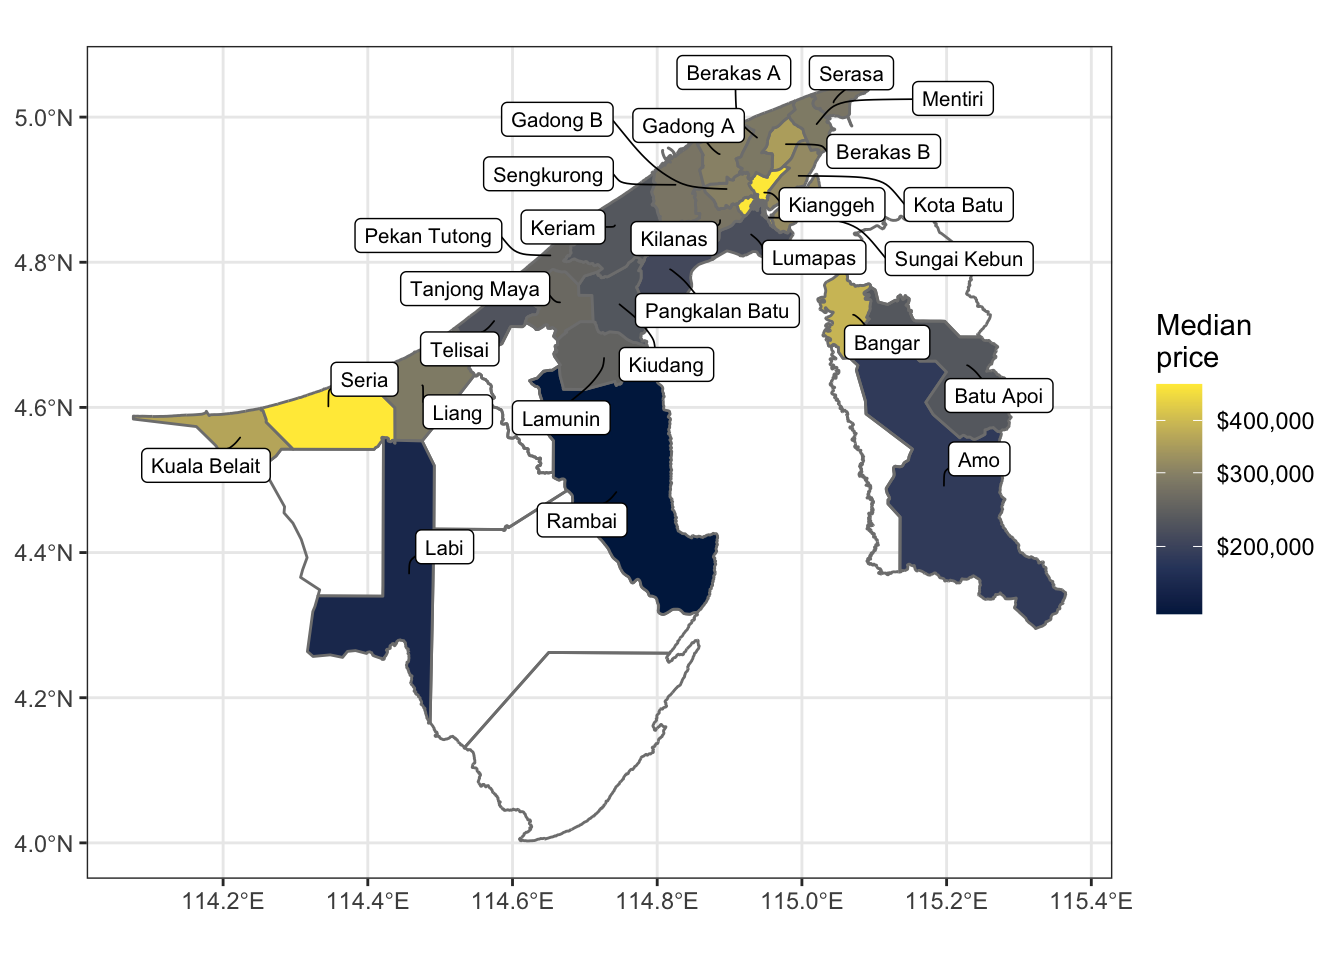
\includegraphics[keepaspectratio]{manuscript_files/figure-latex/notebooks-analysis-fig-spatial-output-2.png}}

}

\caption{\label{fig-spatial}Spatial distribution of median property
prices by mukim.}

\end{figure}%

\textsubscript{Source:
\href{https://Bruneiverse.github.io/house-data/notebooks/analysis-preview.html\#cell-fig-spatial}{Plots
and Data Summaries}}

\subsection{Listing Dates}\label{listing-dates}

The \texttt{date} variable represents the date on which the property
listing was obtained, rather than the date of sale or transaction, and
should be interpreted as a snapshot of market conditions at a specific
point in time. Figure~\ref{fig-price-evolution} illustrates the price
evolution over time. For analysis, we recommend aggregating data by
quarters, as represented by the \texttt{quarter} variable. This
aggregation helps address potential issues like missing data (see
subsection below) and provides a more stable and robust representation
of market trends, making it suitable for temporal analysis of the
housing market.

\begin{figure}[H]

\centering{

\pandocbounded{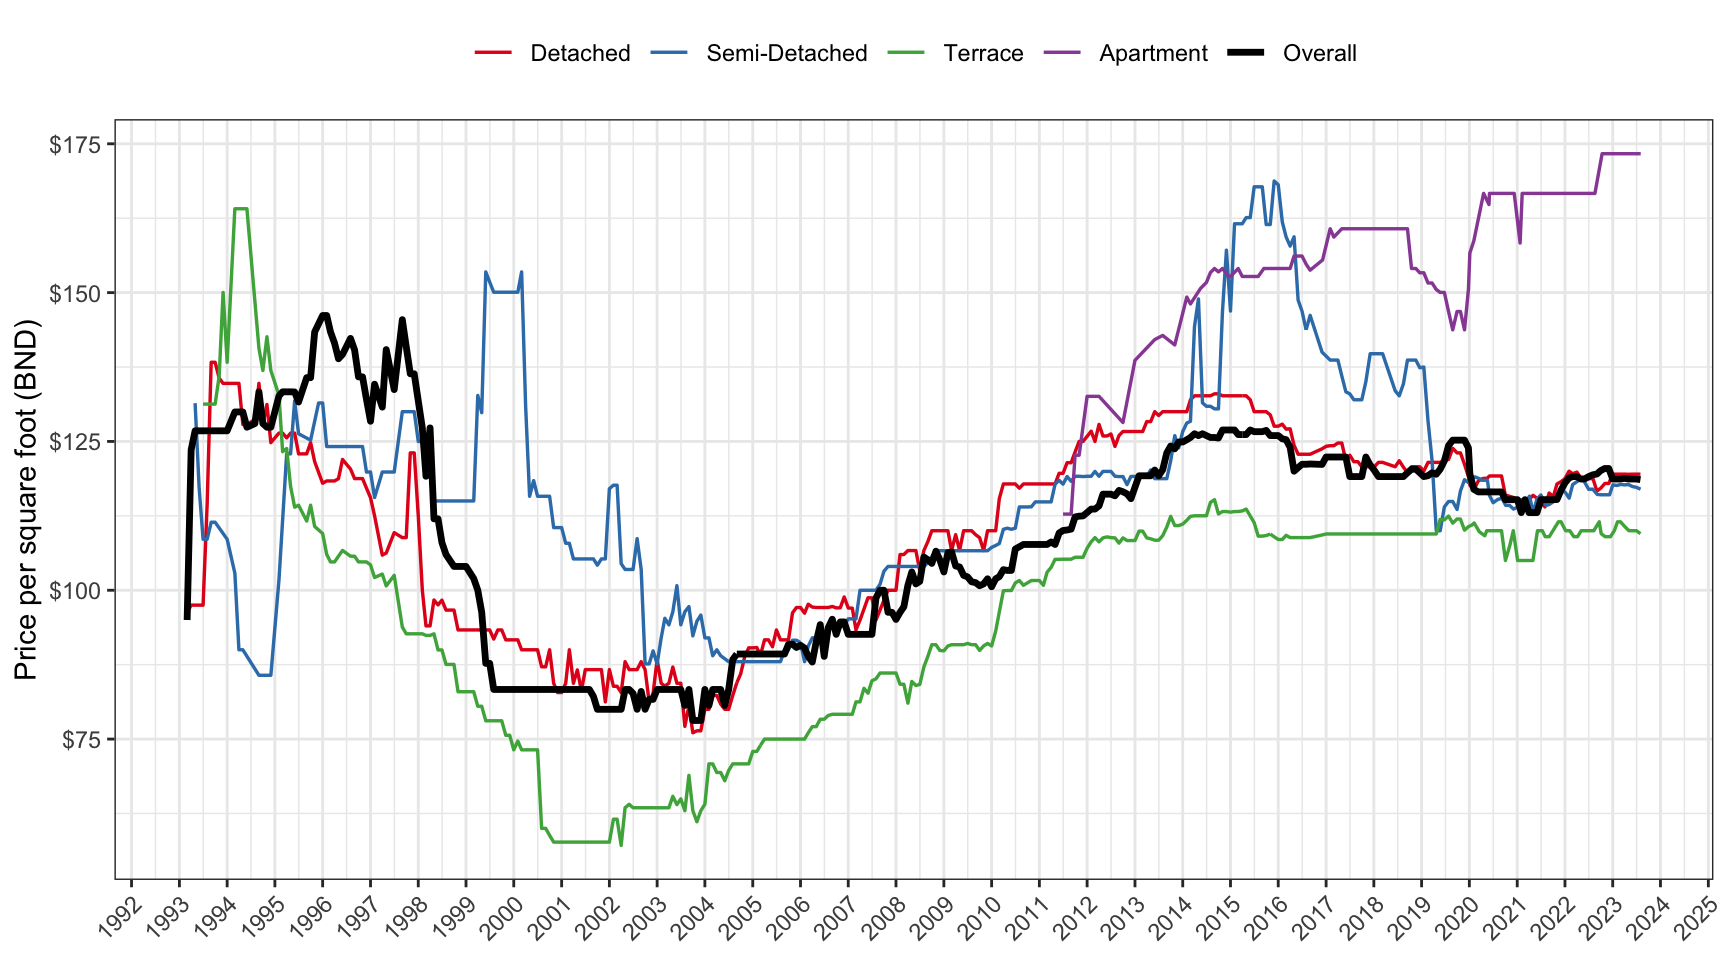
\includegraphics[keepaspectratio]{manuscript_files/figure-latex/notebooks-analysis-fig-price-evolution-output-2.png}}

}

\caption{\label{fig-price-evolution}Median smoothed prices per square
foot by property type using a 24-month (8-quarter) rolling window.}

\end{figure}%

\textsubscript{Source:
\href{https://Bruneiverse.github.io/house-data/notebooks/analysis-preview.html\#cell-fig-price-evolution}{Plots
and Data Summaries}}

\subsection{Missing Values}\label{missing-values}

In any data collection effort, it is unsurprising to encounter missing
data. Likewise in our data set, missing values occur across several
property characteristics--such as plot area, floor area, beds, baths,
and others. A preliminary analysis of the missing data patterns
indicates that the missingness is not completely random, with certain
variables displaying dependencies on others. Advertisers often include
only the information they deem most marketable or necessary, while other
details may be omitted if they are considered standard or implied. For
instance, a listing might specify the square footage and price but leave
out the number of bedrooms and bathrooms, assuming that prospective
buyers are able to infer these details.

\begin{figure}[H]

\centering{

\pandocbounded{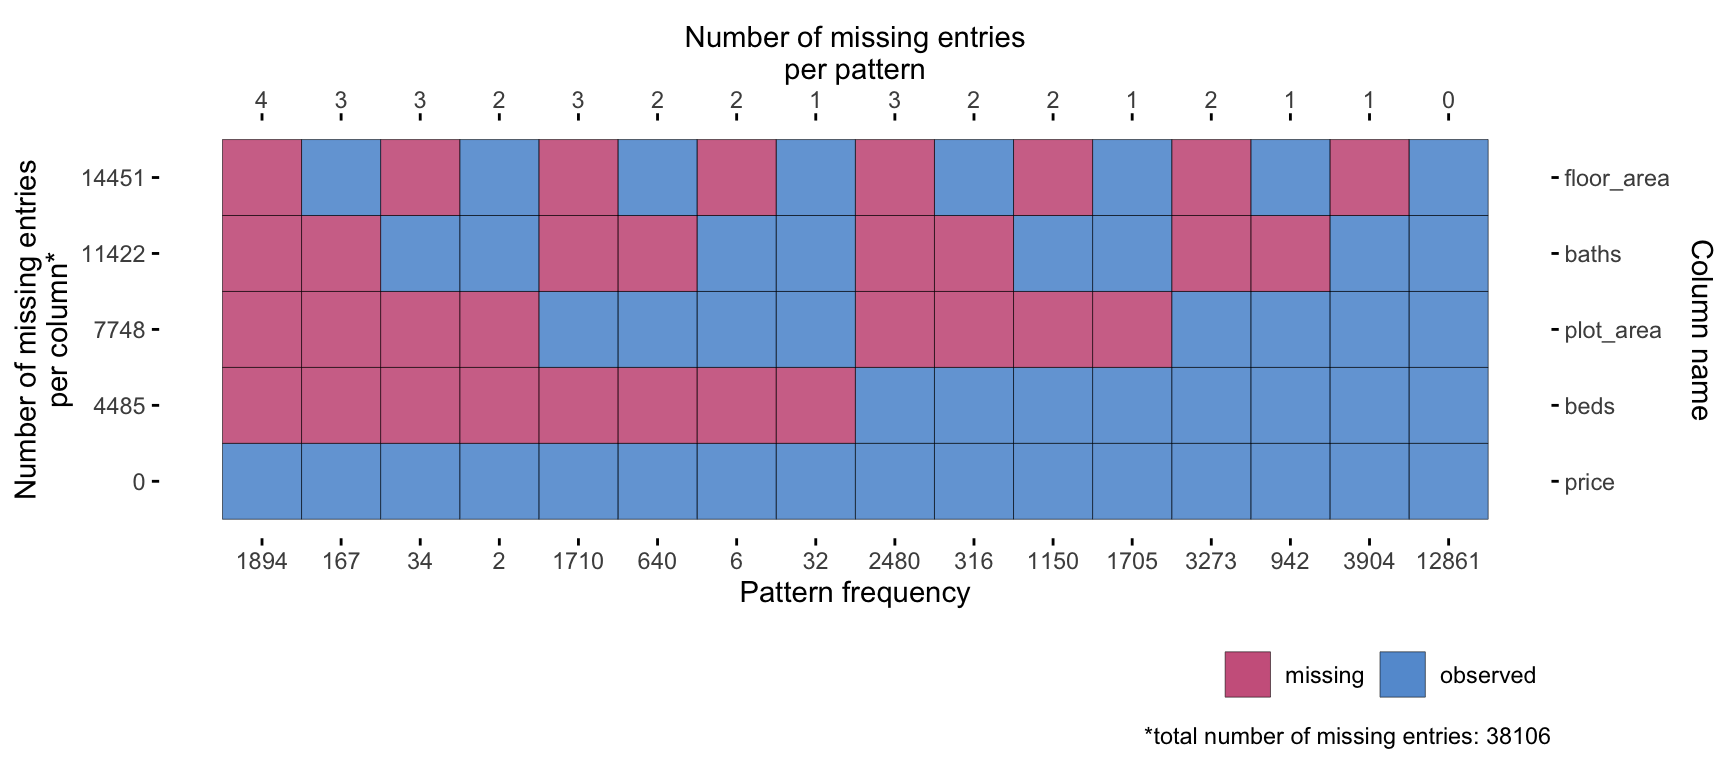
\includegraphics[keepaspectratio]{manuscript_files/figure-latex/notebooks-missing-fig-missing-pattern-output-2.png}}

}

\caption{\label{fig-missing-pattern}Missing data patterns for key house
characteristics.}

\end{figure}%

\textsubscript{Source:
\href{https://Bruneiverse.github.io/house-data/notebooks/missing-preview.html\#cell-fig-missing-pattern}{Missing
Data Patterns}}

Missing values are represented by blank cells in the CSV file. The
severity of missingness is summarised in Table~\ref{tbl-avail} and
patterns visualised in Figure~\ref{fig-missing-pattern}. In total,
10.1\% of the records contain missing values for all key house
characteristics (i.e.~plot area, floor area, beds, and baths), which,
depending on the research question, may require imputation or the
exclusion of these records.

\section{Experimental Design, Materials and Methods}\label{sec-method}

In this section we describe the data collection process, which involved
either a manual transcription of property listings from newspapers, or
web scraping of online property agent listings. The data collection
method varied over the years due to the availability of data sources and
the evolution of technology. For the later years, a large language model
(LLM) was also employed to perform data cleaning on the web scraped
data. Table~\ref{tbl-avail} details which method was used for each year
in the data set, and whether the data was subjected to LLM
post-processing.

All analyses were conducted using the R programming language
\citep{rcoreteam2024language}, with specific packages used described in
each subsection below.

\begin{table}

\caption{\label{tbl-avail}Data availability by year.}

\centering{

}

\end{table}%

\textsubscript{Source:
\href{https://Bruneiverse.github.io/house-data/notebooks/analysis-preview.html\#cell-tbl-avail}{Plots
and Data Summaries}}

\subsection{Manual Data Collection}\label{manual-data-collection}

Early years data collection was conducted manually, involving the
transcription of property listing details from advertisements into a
digital tabular format. This process was carried out by two of the
authors over a period of nine months, from October 2023 to July 2024,
working at a manageable pace. A total of 12,092 data points were
collected in this manner, which translates to processing approximately
150 entries per week per person. Spreading the task over such an
extended period ensured that transcribers were never under time
pressure, which could have led to errors due to fatigue.

The primary sources of the property listings were local newspapers and
magazines. Physical copies were accessed through the National Archive of
Brunei Darussalam, while digital versions, which are digitised replicas
of the physical newspapers, were obtained online. These digital formats
were not structured in a way that allowed for automated scraping, hence
the need for manual transcription.

Although daily newspapers from 1993 onward were available at the
National Archive, the classified sections were not always present. From
1993 to 1999, property advertisements were found only in Friday
editions, and occasionally on Saturdays. Thus, newspapers from both
these days were reviewed weekly to capture the listings data. This
yielded roughly between 300 and 700 listings per year.

From the year 2000 onwards, property advertisements were published daily
in the classifieds section. However, reviewing every single daily
edition was not practical and would increase the likelihood of recording
duplicate listings, thus necessitating a sampling strategy. The sampling
was done as follows. Three newspaper editions per week were selected,
and the classifieds section was reviewed for property listings. When a
listing was found, it was recorded after careful filtering to ensure it
was unique. This manual filtering process involved cross-checking based
on the real estate agent, house characteristics, price, location, and
date proximity. To avoid duplication, the same house listing was not
recorded more than once within a quarter. This process yielded roughly
the same number of listings per year as the earlier years.

\subsection{Web Scraping}\label{web-scraping}

To compile additional property data for the study beyond manual data
collection, web scraping was employed using the R programming language,
making use of the \texttt{\{rvest\}} package \citep{wickham2024rvest}.
This method enabled the systematic extraction of structured information
from various local property listing websites such as panvilla.com (now
defunct), bruhome.com, and bruneiproperty.com.bn. Such websites provide
extensive details on properties listed as ``for sale'' in Brunei,
aggregating advertisements from real estate agents and property
developers.

\begin{figure}

\begin{minipage}{\linewidth}

\centering{

\pandocbounded{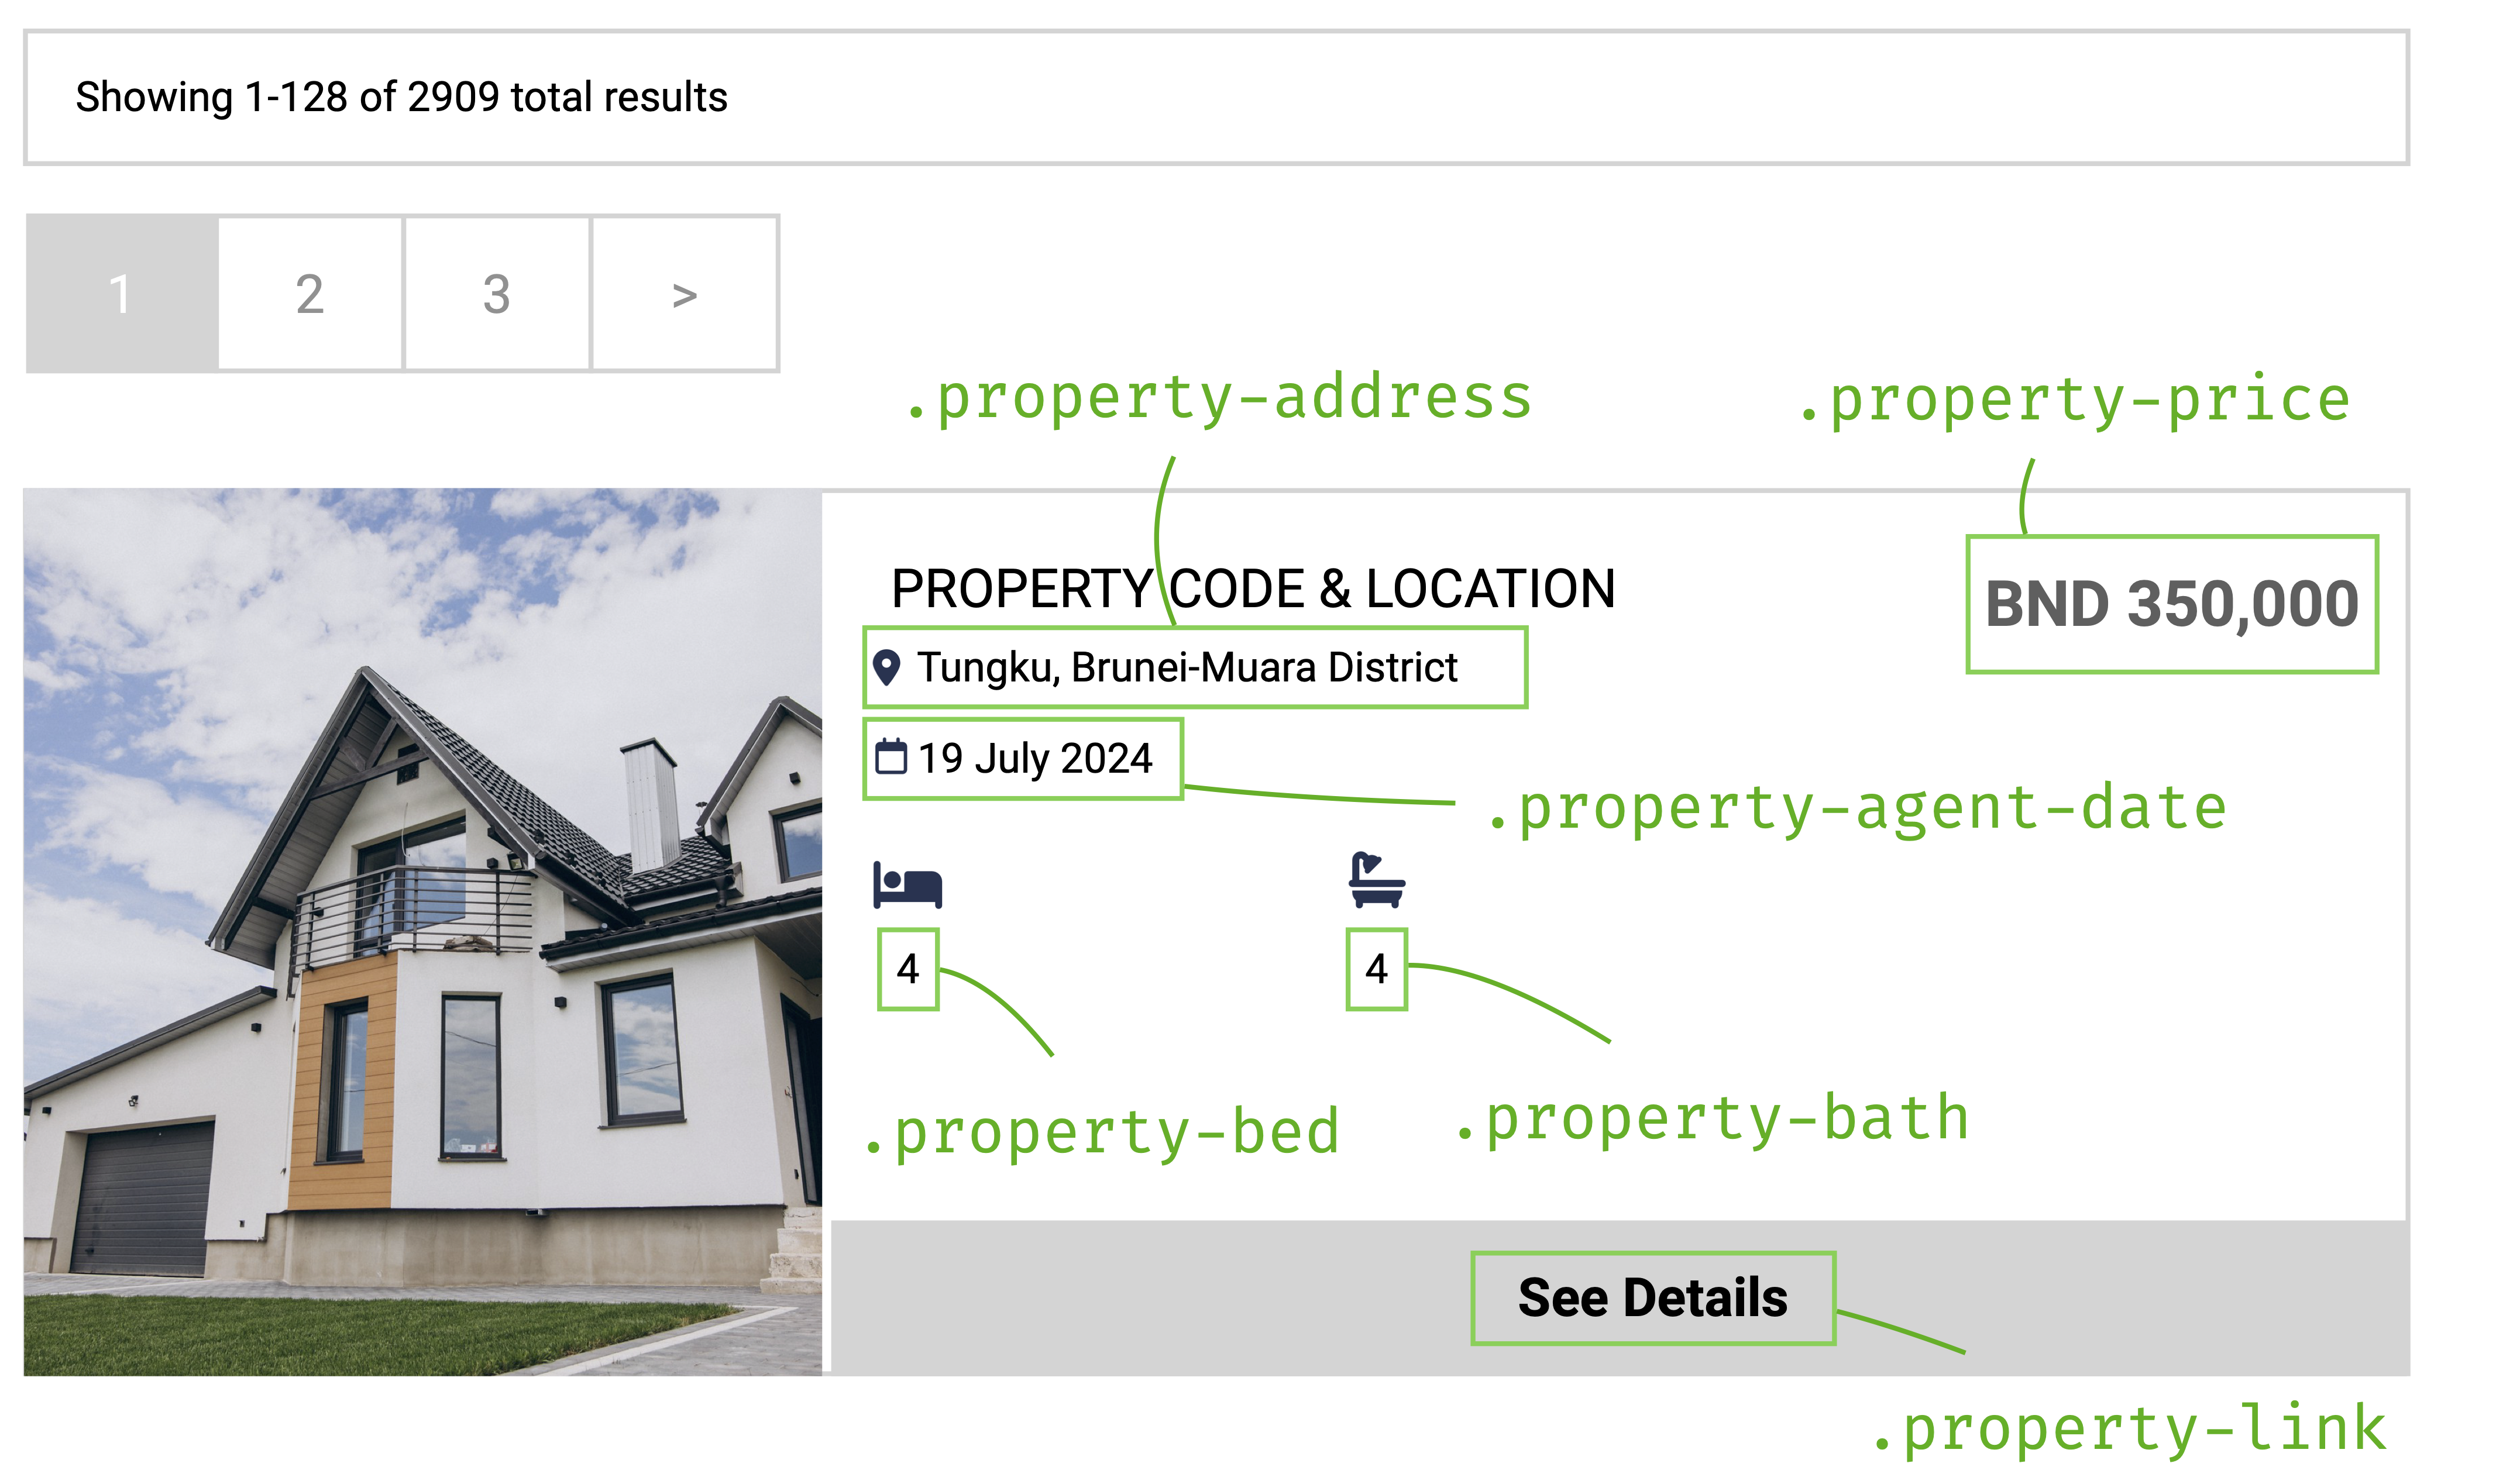
\includegraphics[keepaspectratio]{figures/house-mockup1.png}}

}

\subcaption{\label{fig-mockup-listing}}

\subcaption{\label{}A mockup of the structure of property listing
showing various HTML elements.}
\end{minipage}%
\newline
\begin{minipage}{\linewidth}

\centering{

\pandocbounded{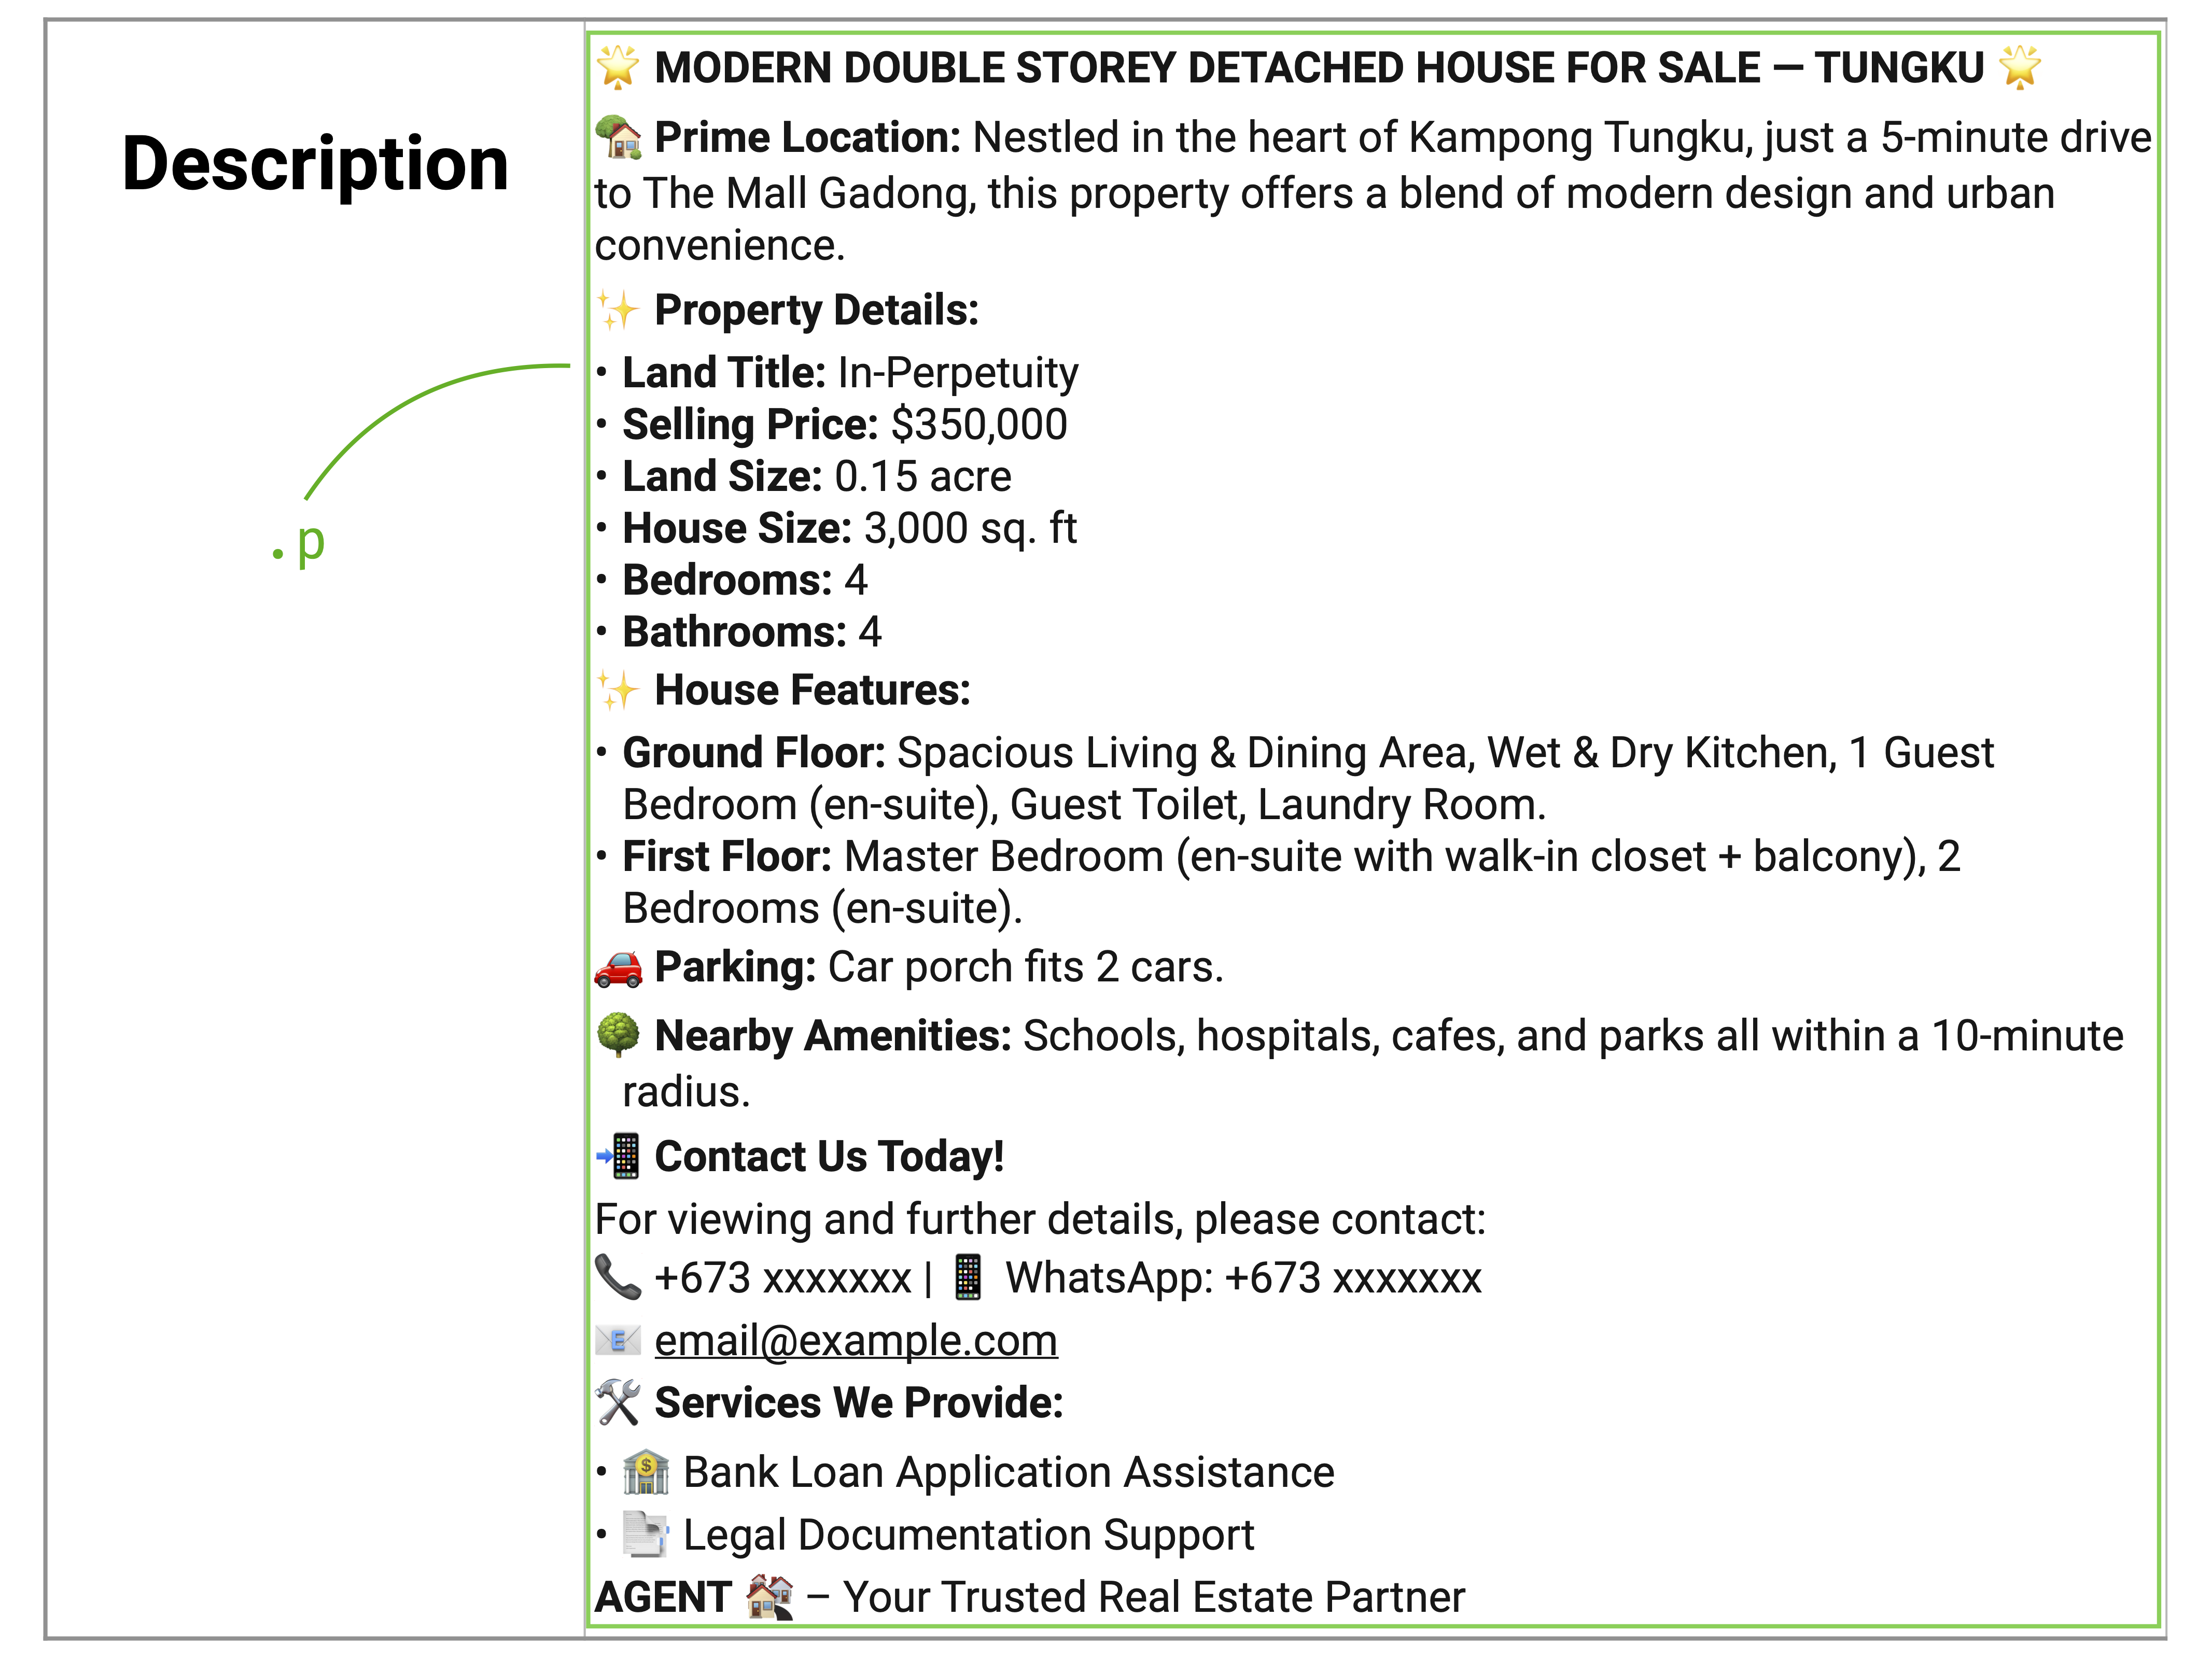
\includegraphics[keepaspectratio]{figures/house-mockup2.png}}

}

\subcaption{\label{fig-mockup-table}}

\subcaption{\label{}Example paragraph containing description within the
``See Details'' link for each property.}
\end{minipage}%

\caption{\label{fig-web-scrape}Illustration of a property listing from a
typical Bruneian property portal. Attribution: Freepik.}

\end{figure}%

The process began by identifying the structure of the target websites,
focusing on the HTML tags and classes containing the relevant
information. The goal here is to programmatically pinpoint and collect
specific information like text, links, or attributes. For example,
elements such as property prices, number of bedrooms, bathrooms,
location, and other features were enclosed within specific HTML
elements, which \texttt{\{rvest\}} functions like
\texttt{html\_elements()} and \texttt{html\_text2()} could target and
extract efficiently. Figure~\ref{fig-mockup-listing} illustrates the
structure of a typical property listing showing the various HTML
elements to target. Example code to perform this task in available in
the repository.

Each webpage displayed a fixed number of listings (e.g.~128 per page).
To scrape all pages, a loop was created to iterate through each page by
modifying the URL (such as with an
\texttt{\&offset=\textless{}number\textgreater{}} parameter, where
\texttt{\textless{}number\textgreater{}} represents the cumulative
number of listings already scraped).

Extracted data required some cleaning to standardise formats for
analysis. Specifically:

\begin{itemize}
\tightlist
\item
  \texttt{price} variables were cleaned by removing non-numeric
  characters and converted to integers.
\item
  \texttt{beds} and \texttt{baths} were converted to integers.
\item
  \texttt{date} variables were formatted properly as \texttt{Date}
  objects.
\item
  Locations were stored as text strings. See the subsection below on
  spatial data harmonisation.
\item
  Any additional information was extracted from the property
  descriptions and saved as a character vector. This very often
  contained valuable insights not captured in the primary fields.
\end{itemize}

Data from 2012 up until the present (February 2025) were managed to be
collected using this method, averaging around 1,500 listings per year.
While highly efficient, this process relied heavily on the consistency
of the site structure of the source webpages. Changes to website layouts
or closures over time required significant updates to the scraping
scripts. To overcome these issues, alternative approaches, such as using
Large Language Models (LLMs), were considered. This is explained in the
next subsection.

\subsection{LLM Data Extraction}\label{llm-data-extraction}

As previously mentioned, the web scraping process also captured
unstructured information from the property descriptions, which often
contained valuable details not captured in the primary fields. In this
subsection, we detail the data extraction process using a pre-trained
Large Language Model (LLM) to extract structured information from the
unstructured text. The LLM used was the DeepSeek R1 distilled Qwen 14B
\citep{deepseek2025deepseekr1, qwen2025qwen25}, accessed using the
\texttt{\{ellmer\}} R package \citep{wickham2025ellmer} via the
Ollama\footnote{\url{https://github.com/ollama/ollama}} API, a local
interface platform to the LLM.

The primary goal was to extract the house characteristics of interest,
specifically variables 7 to 15 as per Table~\ref{tbl-codebook}, from the
unstructured verbose descriptions scraped from property listing
websites. Each description was processed with a carefully crafted prompt
(Figure~\ref{fig-llm-prompt}) to ensure consistent output. This prompt
instructed the model to return only the required information in a
semicolon-separated format, while handling edge cases such as missing
descriptions or non-residential (commercial) properties.

\begin{figure}

\centering{

\begin{Shaded}
\begin{Highlighting}[]
\StringTok{"The following is the description from a property sale listing in Brunei. This }
\StringTok{description will contain the information about the property, including its }
\StringTok{characteristics, price, and location. However, some of these descriptions may }
\StringTok{not contain property listings, and instead contain other or no information at }
\StringTok{all.}

\StringTok{In the case where this description is in fact a property listing, I would like }
\StringTok{you to extract the following information:}

\StringTok{1. Location / area of the property in Brunei, CHARACTER.}
\StringTok{2. Price of the property in Brunei Dollars, NUMERIC.}
\StringTok{3. Type of property, CHARACTER {-}{-} select from Detached, Semi{-}Detached, Terrace, }
\StringTok{Apartment, or Land.}
\StringTok{4. Land tenure, CHARACTER {-}{-} select from Freehold, Leasehold, or Strata. If }
\StringTok{other than this, return \textquotesingle{}NA\textquotesingle{}.}
\StringTok{5. Status of the property, CHARACTER {-}{-} select from Proposed, Under }
\StringTok{Construction, New, or Resale.}
\StringTok{6. Land area in acres, NUMERIC.}
\StringTok{7. Built up area in square feet, NUMERIC.}
\StringTok{8. Number of storeys, INTEGER.}
\StringTok{9. Number of bedrooms, INTEGER.}
\StringTok{10. Number of bathrooms, INTEGER.}

\StringTok{Further instructions:}

\StringTok{{-} Please return **semicolon** separated values like this:}

\StringTok{  Kg Tanah Jambu; 250000; Detached ; Freehold ; New     ; 0.3 ; 2500; 2;  3; 3}
\StringTok{  Kg Tungku     ; 300000; Terrace  ; Leasehold; Resale  ; 0.25; 1700; 2;  3; 2 }
\StringTok{  Kg Kiarong    ; 200000; Apartment; Strata   ; Proposed; 0.1 ; 1000; NA; 2; 2}
\StringTok{  etc.}
\StringTok{  NUMBERS SHOULD NOT CONTAIN comma (,) for thousands separator}

\StringTok{{-} If any of the 10 values are missing, please return \textquotesingle{}NA\textquotesingle{} for that value.}

\StringTok{{-} If the description does not contain a property listing (for example, it is a }
\StringTok{rental property advertisement), return \textquotesingle{}NA\textquotesingle{} for all 10 values.}

\StringTok{{-} DO NOT RESPOND WITH ANYTHING ELSE OTHER THAN THE REQUIRED INFORMATION."}
\end{Highlighting}
\end{Shaded}

\textsubscript{Source:
\href{https://Bruneiverse.github.io/house-data/manuscript-preview.html}{Article
Notebook}}

}

\caption{\label{fig-llm-prompt}The LLM prompt to clean descriptions
obtained from web scraping.}

\end{figure}%

The verbose descriptions were fed into the model one at a time using a
loop, with the LLM extracting and returning the relevant details. Note
that this loop was not parallelised, as the LLM already utilises
multiple cores, and further parallelisation would not yield significant
efficiency gains due to resource constraints. The cleaned results were
then parsed and stored in a data frame, which was then subjected to
manual data-type validation to ensure conformity with the existing data
set (see the last subsection). It takes, on average, 81.7 seconds to
process a single description using a Mac Pro 3.2GHz 16 core Intel Xeon W
with 48GB of DDR4 RAM. We processed 5,055 descriptions from 2020 to 2025
using this method, with a run time of approximately 20 hours in total
spread over three machines.

To evaluate the accuracy of the LLM data extraction, a test data set of
100 artificially generated descriptions was created, with each
description written in the style of a typical property listing. For each
house characteristic, the accuracy of the LLM was calculated by
comparing the extracted value to the ground truth. For numeric
variables, values were considered accurate if they fell within 1\% of
the corresponding ground truth value. For character variables, accuracy
was determined using the normalised Levenshtein distance, ensuring
differences remained within a set threshold. The test data also
contained missing information in certain property characteristics, which
the LLM was expected to handle correctly. A correct handling was counted
if both the extracted and ground truth values were missing. Accuracy was
then averaged per characteristic as well as across all characteristics.

Our experiments show that the LLM data extraction process with the
deepseek-r1:14b model achieved an overall accuracy rate of 96.9\% (see
Appendix for complete results). Errors mostly stemmed from incorrect
\texttt{status} classification, likely due to the vagueness of the
advertisement listing. As for the rest of the variables, clear errors
were flagged and corrected manually during our data validation process
(described in the subsection following the next one). Overall, the LLM
was found to be a valuable tool for extracting structured information
from unstructured text, significantly reducing the time and effort
required for data extraction.

\subsection{Spatial Data Harmonisation}\label{sec-spatial-harm}

Whether the data was collected manually, through web scraping, or
cleaned using the LLM, the spatial information extracted was often
inconsistent in terms of naming conventions and granularity. To address
this, a spatial data harmonisation process was conducted to standardise
the names of the kampongs (villages) in the data set to the format used
by Department of Economic Planning and Statistics (DEPS), Ministry of
Finance and Economy, Brunei Darussalam as per the most recent census
\citep{deps2022population}. This is the same format used by the R
package \texttt{\{bruneimap\}} \citep{jamil2024bruneimap}. The CSV file
\texttt{bn\_kpg\_level\_data.csv} obtained from this package was used as
a reference to standardise the kampong names in the data set, which
conveniently also includes the mukim and district names for each
kampong.

The majority of house listings in Brunei specify the property location
using the kampong name, the smallest administrative unit in the country.
The task in hand was then to match these kampong names in the data set
with the standardised names in the reference file. Several challenges
were encountered during this process, including:

\begin{enumerate}
\def\labelenumi{\arabic{enumi}.}
\tightlist
\item
  Spelling variations and misspellings, though these were relatively
  straightforward to correct.
\item
  Unknown entries, where the correct kampong could sometimes be inferred
  from the geographical context; otherwise, these were set to
  \texttt{NA}.
\item
  Multiple matches, occurring when two or more kampongs shared the same
  name (e.g., Kampong Panchor in Mukim Mentiri and Kampong Panchor in
  Mukim Lumapas). Additional information from the listing was used to
  determine the correct match, but where this was not possible, these
  entries were also set to \texttt{NA}.
\end{enumerate}

This process was carried out manually using data filtering features in
Microsoft Excel. Once completed, all entries marked as \texttt{NA} were
removed so as to provide complete spatial coverage for the data set.

\subsection{Data Validation}\label{sec-data-validation}

To ensure data quality, a series of consistency and validity checks were
performed on the data set, especially after manual transcription and LLM
data cleaning. These checks include:

\begin{enumerate}
\def\labelenumi{\arabic{enumi}.}
\tightlist
\item
  \textbf{Outlier detection.} Statistical summaries were analysed to
  identify and flag anomalous values. For instance, a built-up area
  recorded as 0.1 square feet or an implausibly high number of beds and
  baths (e.g., \textgreater20) would likely indicate an error, prompting
  review. Such anomalies were flagged and manually reviewed for
  correction.
\item
  \textbf{Internal consistency checks.} This made use of substantive
  knowledge about Brunei's housing market
  \citep{jamil2025spatiotemporal}. An example is using the price per
  square foot indicator, whose value typically falls within a known
  range. Therefore any deviations were scrutinised to ensure that
  variables such as price and floor area were correctly recorded. This
  was similarly applied to other variables such as plot area, beds, and
  baths.
\item
  \textbf{Duplicate records detection.} We also performed duplicate
  record detection to identify any repeated entries that might have
  arisen from overlapping data sources or transcription errors. Any
  duplicates that were identified were carefully reviewed and removed to
  ensure that each property listing was uniquely represented in the span
  of one calendar month.
\end{enumerate}

These data validation procedures collectively contribute to a robust and
reliable data set, providing a solid foundation for subsequent analysis.

\section*{Limitations}\label{limitations}
\addcontentsline{toc}{section}{Limitations}

Listing prices in our data set serve as a proxy for market values,
capturing advertised trends rather than final sale outcomes. While this
allows for timely analysis of market sentiment, actual transaction
prices may differ due to negotiation dynamics, seller strategies, and
broader market conditions.

Despite significant efforts to ensure data quality, some limitations
remain. First, integrating historical data from manually transcribed
sources with later web-scraped data may introduce inconsistencies,
potentially affecting comparability over time. Second, although
duplicate listings were carefully reviewed and removed, there remains a
slight possibility of residual duplicates within the data set. Thirdly,
while we have confidence in the data quality from 2015 to 2024, property
price trends between 1993 and 2014 cannot be fully verified.
Nonetheless, this study serves as a valuable starting point. Future
research could benefit greatly from access to administrative transaction
data, which would allow for more comprehensive and accurate analyses.

Finally, while significant effort was made to harmonise spatial data,
matching kampong names to standardised references may not be entirely
error-free. However, aggregation to the mukim level provides a reliable
alternative for spatial analyses, ensuring that the data set remains
valuable for research and analysis.

\section*{Ethics}\label{ethics}
\addcontentsline{toc}{section}{Ethics}

The authors confirm that the current work does not involve human
subjects, animal experiments, or data collected from social media
platforms. The data described in this article were obtained from
publicly available, non-personal, and factual sources, including
physical and digital newspapers and magazines.

Web scraping from local property listings websites was conducted in
compliance with ethical and legal considerations. Specifically, data
were not collected from behind login barriers, and the terms of service
(ToS) for the websites did not explicitly prohibit web scraping.
Furthermore, the \texttt{robots.txt} files for the websites were
reviewed, and any policies outlined there were adhered to.

The data collected consisted exclusively of non-copyrightable factual
information, such as property characteristics and spatial locations, and
excluded any potentially copyrighted content such as images. To ensure
privacy, no personally identifiable information, including specific
property addresses, was scraped nor included in the data set. To this
end, data from the description fields processed by the LLM are not
included in the data set, as they may contain sensitive information such
as contact details and company names. The names of real estate agents
and companies have been anonymised to ensure privacy.

\section*{CRediT Author Statement}\label{credit-author-statement}
\addcontentsline{toc}{section}{CRediT Author Statement}

\begin{itemize}
\tightlist
\item
  \textbf{Haziq Jamil}: Conceptualisation, Methodology, Software, Formal
  analysis, Data curation, Writing-Original Draft, Visualisation,
  Supervision, Project administration, Funding acquisition.
\item
  \textbf{Amira Barizah Noorosmawie}: Software, Data curation,
  Writing-Original Draft.
\item
  \textbf{Hafeezul Waezz Rabu}: Software, Data curation,
  Writing-Original Draft.
\item
  \textbf{Lutfi Abdul Razak}: Conceptualisation, Validation,
  Supervision, Funding acquisition.
\end{itemize}

\section*{Acknowledgements}\label{acknowledgements}
\addcontentsline{toc}{section}{Acknowledgements}

The authors gratefully acknowledge the contributions of Atikah Farhain
Yahya, Nurulhanisah Abdul Manan, and Nina Zuhairi for their assistance
in collecting and processing the data presented in this study. The
authors also extend their thanks to the Brunei Darussalam Central Bank
(BDCB) for engaging discussions and valuable support, which were
instrumental in initiating this project.

\section*{Declaration of Competing
Interests}\label{declaration-of-competing-interests}
\addcontentsline{toc}{section}{Declaration of Competing Interests}

The authors declare that they have no known competing financial
interests or personal relationships that could have appeared to
influence the work reported in this paper.

\section*{References}\label{references}
\addcontentsline{toc}{section}{References}

\renewcommand{\bibsection}{}
\bibliography{refs-HJ.bib}

\section*{Appendix}\label{appendix}
\addcontentsline{toc}{section}{Appendix}

\subsection{Pairwise Correlation Plot of Numeric
Variables}\label{pairwise-correlation-plot-of-numeric-variables}

Figure~\ref{fig-corr} shows the pairwise correlation plot of the numeric
variables in the data set.

\begin{figure}[H]

\centering{

\pandocbounded{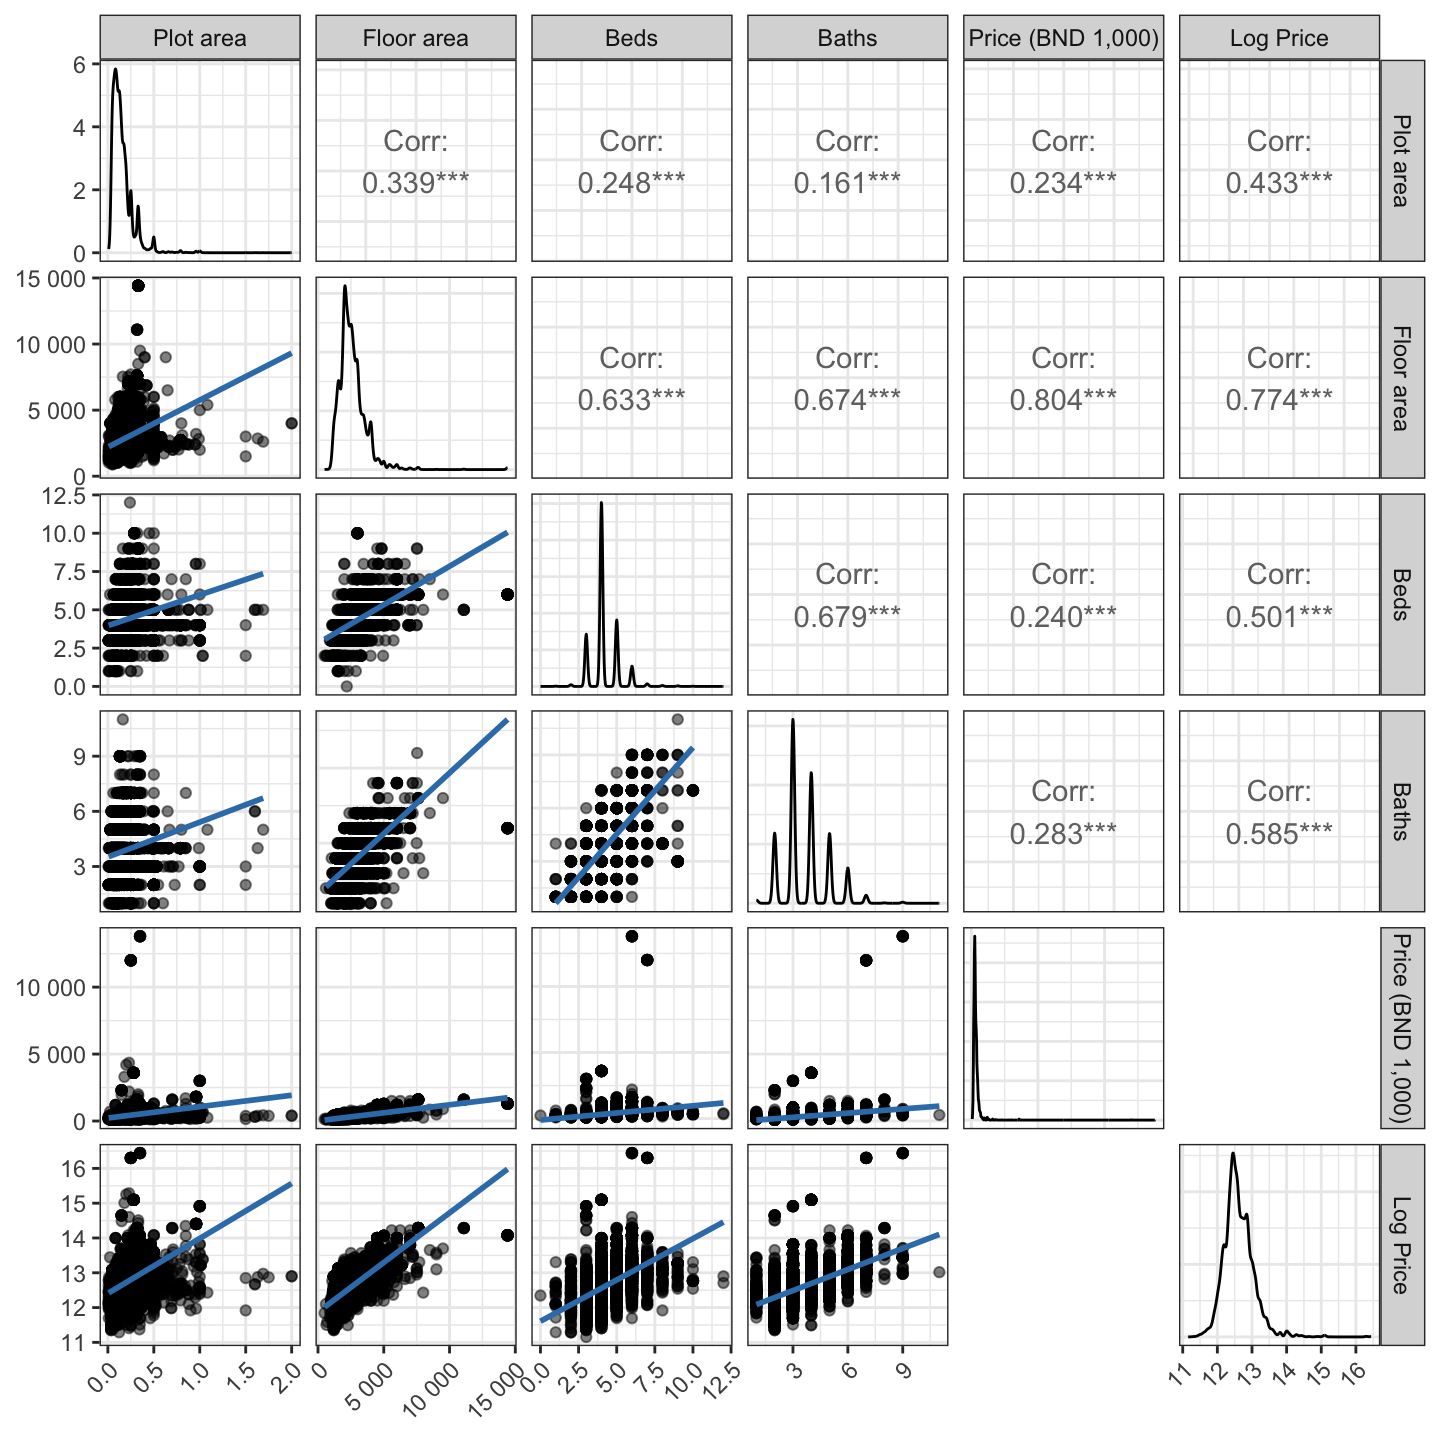
\includegraphics[keepaspectratio]{manuscript_files/figure-latex/notebooks-analysis-fig-corr-output-2.png}}

}

\caption{\label{fig-corr}Pairwise correlation plot of continuous
variables.}

\end{figure}%

\textsubscript{Source:
\href{https://Bruneiverse.github.io/house-data/notebooks/analysis-preview.html\#cell-fig-corr}{Plots
and Data Summaries}}

\subsection*{Comparison to RPPI Data}\label{comparison-to-rppi-data}
\addcontentsline{toc}{subsection}{Comparison to RPPI Data}

To demonstrate the quality of the data set, we compared it with the
Residential Property Price Index (RPPI) \citep{bdcb2021technical}
published by the Brunei Darussalam Central Bank (BDCB). A simple median
price per square foot (PPSF) index can be calculated by aggregating the
data by quarters. This approach minimises the impact of missing values,
as the index is based on aggregated data. Figure~\ref{fig-rppi} shows
the comparison between the RPPI and the PPSF index calculated from our
data set. The mean absolute error (MAE) between the two indices is
calculated to be 4.71\%, indicating a good level of agreement between
the two data sets.

\begin{figure}[H]

\centering{

\pandocbounded{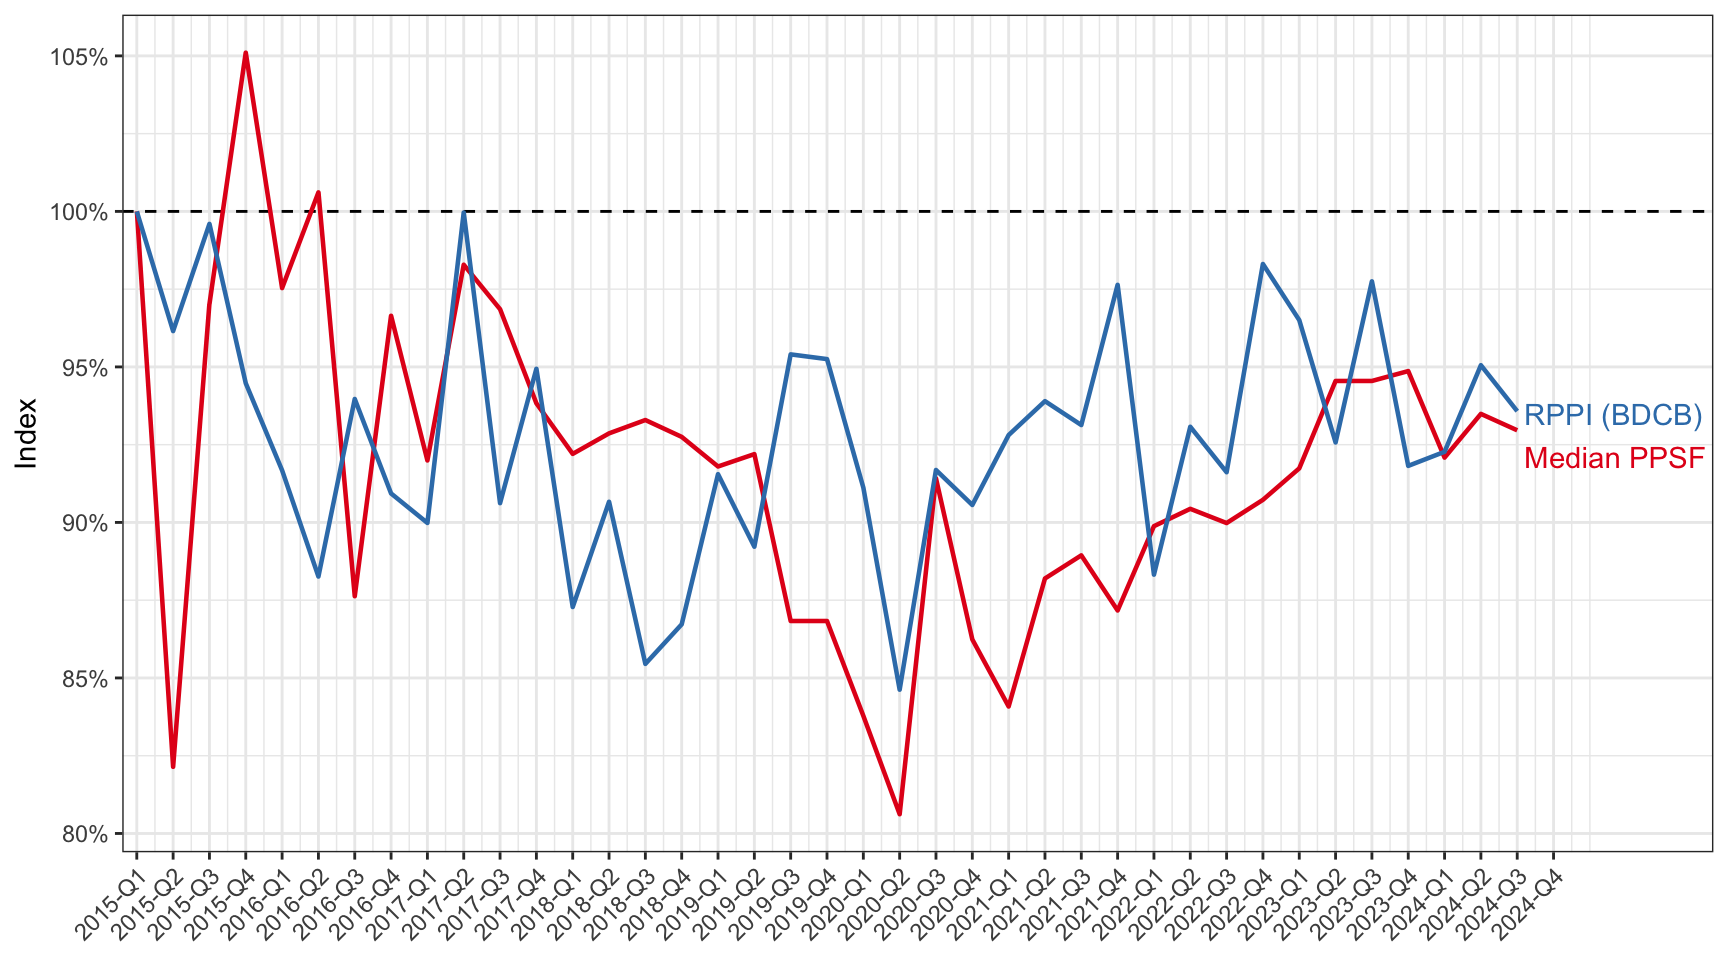
\includegraphics[keepaspectratio]{manuscript_files/figure-latex/notebooks-analysis-fig-rppi-output-1.png}}

}

\caption{\label{fig-rppi}Comparison of quarterly median price per square
foot indices (Median PPSF) and the official Residential Property Price
Index (RPPI) from Brunei Darussalam Central Bank (BDCB).}

\end{figure}%

\textsubscript{Source:
\href{https://Bruneiverse.github.io/house-data/notebooks/analysis-preview.html\#cell-fig-rppi}{Plots
and Data Summaries}}

\subsection*{LLM Accuracy Test}\label{llm-accuracy-test}
\addcontentsline{toc}{subsection}{LLM Accuracy Test}

To test the accuracy of the LLM data extraction, we created a test data
set of 100 house advertisements in the style of the web scraped data.
Several popular models from Ollama were used, namely the Llama3.2 (3B),
Mistral (7B), Phi 4 (14B), and DeepSeek-R1 distilled reasoning models
based on Llama (8B) and Qwen (14B). For the locally run Ollama models,
the settings were set to the default values, with the exception of a
lowered temperature setting: \texttt{temperature\ =\ 0.1},
\texttt{top-p=0.9} (nucleus sampling), \texttt{top-k=40} (top-k
sampling), \texttt{max-tokens=128}, and \texttt{repeat-penalty=1.1}.
Additionally, two models from OpenAI were included for comparison. These
were the GPT-4o and the o1-mini, with the latter being a reasoning
model.

Figure~\ref{fig-llmtest} and Table~\ref{tbl-llmtest-time} show the
accuracy results for each model. OpenAI's models topped the accuracy
charts, with the o1-mini and gpt-4o models achieving the accuracy scores
of 99.2\% and 98.9\% respectively. The reasoning model deepseek-r1:14b
was the best performing locally run model, scoring 96.9\% accuracy.
Evidently, the smaller the model, the less accurate the extraction
process (cf.~llama3.2 70.8\%). Most inaccuracies occurred in the
\texttt{status} variable, where models struggled to parse the correct
build status from vague advertisement descriptions. However, key
variables such as \texttt{price}, \texttt{type}, \texttt{plot\_area},
\texttt{floor\_area}, \texttt{beds}, and \texttt{baths} are generally
reliable (\textgreater90\% accuracy).

\begin{figure}[H]

\centering{

\pandocbounded{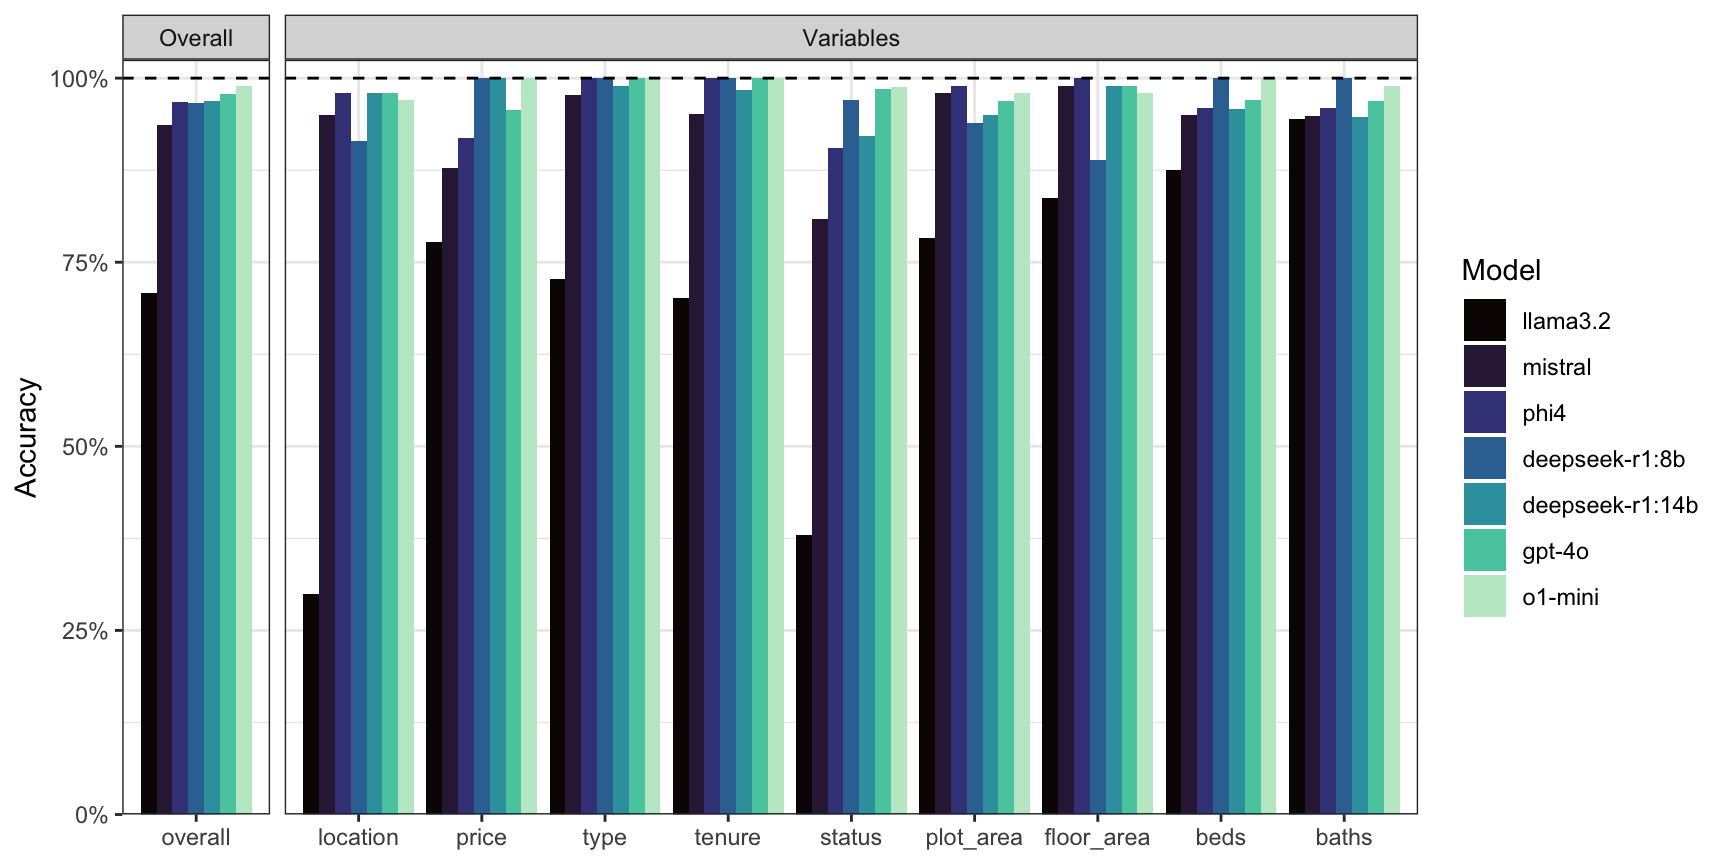
\includegraphics[keepaspectratio]{manuscript_files/figure-latex/notebooks-analysis-fig-llmtest-output-1.png}}

}

\caption{\label{fig-llmtest}Comparison of data extraction accuracy
across multiple LLM models on the test dataset. Each bar represents the
percentage of correctly extracted fields for a given model.}

\end{figure}%

\textsubscript{Source:
\href{https://Bruneiverse.github.io/house-data/notebooks/analysis-preview.html\#cell-fig-llmtest}{Plots
and Data Summaries}}

The run time statistics for each model is shown in the table below. The
computer used was a Mac Pro 3.2GHz 16 core Intel Xeon W with 48GB of
DDR4 RAM. At the time of running the tests, graphics card support was
not available for the LLM models, which would have significantly reduced
the run time. Certainly cloud-based models such as OpenAI's models are
much faster than running models locally, though a paid API key is
required.

\begin{table}

\caption{\label{tbl-llmtest-time}Single run time statistics for LLM data
extraction for each model in seconds.}

\centering{

\fontsize{12.0pt}{14.4pt}\selectfont
\begin{tabular*}{\linewidth}{@{\extracolsep{\fill}}lrrrr}
\toprule
 & \multicolumn{4}{c}{Time (seconds)} \\ 
\cmidrule(lr){2-5}
Model & Minimum & Mean & Median & Maximum \\ 
\midrule\addlinespace[2.5pt]
llama3.2 & 1.08 & 6.40 & 9.60 & 10.16 \\ 
mistral & 2.66 & 10.44 & 2.91 & 22.21 \\ 
phi4 & 3.72 & 14.11 & 4.27 & 38.01 \\ 
deepseek-r1:8b & 36.83 & 65.97 & 54.61 & 112.78 \\ 
deepseek-r1:14b & 40.89 & 117.67 & 81.71 & 151.20 \\ 
gpt-4o & 1.28 & 2.46 & 1.73 & 5.38 \\ 
o1-mini & 5.97 & 7.95 & 7.51 & 9.94 \\ 
\bottomrule
\end{tabular*}

}

\end{table}%

\textsubscript{Source:
\href{https://Bruneiverse.github.io/house-data/manuscript-preview.html}{Article
Notebook}}





\end{document}
